%% ----------------------------------------------------------------------------
%% ----------------------------------------------------------------------------
\documentclass[pdftex,11pt,openright,headsepline]{book}

\usepackage{paralist}		% List environment
\usepackage{color}		% For colored text
\usepackage{times}
\usepackage{amsfonts}		% Additional math fonts
\usepackage{amsmath}		% Math symbols
\usepackage{latexsym}
\usepackage{graphicx}		% For including images
%\usepackage{listings}		% If listings are needed
%\usepackage{mydefs}		% Some of our own definitions
% \usepackage{wrapfig}		% To wrap images
% \usepackage{algorithmic}	% Nice algorithm environment
% \usepackage{algorithm}
\usepackage{fancyhdr}		% Produce the nice header
\usepackage{fullpage}           % Use the full page
\usepackage{url}
\usepackage{amssymb}
\usepackage{mathtools}
\usepackage{setspace}
\doublespacing
\usepackage{xspace}
\usepackage{etoolbox}
\usepackage{enumitem}

\usepackage[final]{pdfpages}

\setlength{\headsep}{10mm}


% Change the appearance of the header. Here \MakeUppercase is hard-coded, so renewing this command allows to elegantly change the header appearance.
\renewcommand{\MakeUppercase}{\scshape}

% Set the headings' appearance in the ``fancy'' pagestyle
\fancyhead{}
\fancyhead[RO, LE]{\leftmark}
\fancyfoot{}
\fancyfoot[RO, LE]{\thepage}

% The first pages shall be empty, even no page numbering 
\begin{document}
\pagestyle{empty} % even no page number

\fancypagestyle{plain}{
  \renewcommand{\headrulewidth}{0.0pt}
  \fancyfoot{}
  \fancyhead{}
}


% Title page, modify accordingly 
%% ----------------------------------------------------------------------------
% BIWI SA/MA thesis template
%
% Created 09/29/2006 by Andreas Ess
% Extended 13/02/2009 by Jan Lesniak - jlesniak@vision.ee.ethz.ch
%% ----------------------------------------------------------------------------

\begin{titlepage}

\thispagestyle{empty}

\fancypagestyle{empty}{
\lhead{
\includegraphics[height=1.5cm]{images/ethlogo_black}}
\renewcommand{\headrulewidth}{0.0pt}
\rhead{\vspace*{-0.2cm}
\includegraphics[height=1.4cm]{images/zhaw_sml.png}}
\fancyfoot{}
}

%% Document information

\vspace*{2cm}
\begin{center}
\Huge{\textbf{Does the trend towards indexation cause market instability?}\\}
\LARGE{\textbf{}\\[1cm]}

\large{Master Thesis\\[0.8cm]}
\LARGE{Apoorva Gupta\\}
\normalsize{Department of Banking and Finance, ZHAW}
\end{center}

% \begin{center}
% \begin{center}
% \begin{tabular}{ll}
% \multirow{2}{*}{
\includegraphics[height=1cm]{images/biwi_logo}} & Computer Vision Laboratory\\ 
% & ETH Zurich
% \end{tabular}
%  \end{center}
% \end{center}


\vfill
\begin{center}
\begin{tabular}{ll}
\Large{\textbf Advisor:} & \Large{Dr. Qunzhi Zhang, ETH Zurich}\\
\Large{\textbf Supervisor:} & \Large{Prof.~Dr.~Oliver Bachmann, ZHAW}\\
							& \Large{Prof.~Dr.~Didier Sornette, ETH Zuirch}\\
% 			    & \small{Computer Vision Laboratory}\\
% 			    & \small{Department of Information Technology and Electrical Engineering}\\
\end{tabular}
\end{center}

\end{titlepage}

\cleardoublepage

%% ----------------------------------------------------------------------------

\newpage
\vspace{3cm}

\chapter*{Abstract}

``The next crash risk is hiding in plain sight-Sometimes the ticking time bomb is in corners of the system that seem dull and safe''- says Gillian Tett. Sometimes market shocks and bubble occurs because of risky bets like Long-Term Capital Management (LTCM) fund crisis (1987), Portfolio insurance debacle (2007), Quant crisis, Lehman brother bankruptcy in 2008 or the recent house bubble. This situation may be further aggravated in the next decades by the increase in the financialization through Exchange traded funds (ETFs), speed and automation through algorithm trading, and public debt \cite{a5}. The adverse effect of the crisis has lead to a massive exodus of most of the clients, devaluation of the assets, instability in the market, break down in pricing mechanism of the stock market and so on so forth. Today, western banks are well capitalized and regulated by Basel terms. And the economy is flushed with the cash and seems to be calm which reflects a sense of security. But this calmness will not only lead to the danger of risky bets but also for the pearls of safe assets too. 

Even though ETFs led to the Great Crash, but still they are considered to be safe investments. This sector has recently exploded in size with more than 4 billion in asset under management (AUM). Passive and quantitative investors have covered more than 60\% of the AUM, which was under 30\% a decade ago. De planta \cite{a3} has concluded, ``If the majority of us embrace them, index-trackers threaten to sabotage the entire economic system''. This inclination towards passive investment is due to higher fees charged by the active managers and they have underperformed in past decades. Therefore, in order to maintain balance in the economy and outperform the passive investments in the market, active fund managers fight back against ‘Darwinian cull’. Active managers turn to strategies that are difficult to replicate in a passive format. 

This motivated us to develop a new model to help active managers to outperform in the market. We developed a Statistical Agent-Based model (SABM) to solve the problem at hand. The strength of SABM lies in its capability to shift the regime from microscopic to macroscopic level and thus, resolving the complex economic problems. The strategy is to benefit from the tail risk which emanates from crowding which is not adequately priced. In this thesis, we describe the steps for developing a SABM model and formulate the calibration of the model as an optimization problem. The ease of calibrating a model in case of SABM provides an advantage over the use of ABMs. 

Finally, the model is evaluated using historical S\&P 500 index data. We evaluate our model using random trading strategies and linear regression. Various experiments with different window lengths for calibration are used. The preliminary results encourage the prediction and, also conclude that the model provides relevant information. The research findings of this thesis can be used by the active managers in the industry to scientifically justify their business model. It will also help the agents to view the effect of market factors globally.

% Input here any acknowledgements
%% ----------------------------------------------------------------------------
%% ----------------------------------------------------------------------------
\chapter*{Acknowledgements}
I would like to acknowledge the support of my master thesis advisor Dr. Qunzhi Zhang, Post-Doc. at D-MTEC in ETH. I would like to offer my special thanks to Prof. Oliver Bachmann, ZHAW and Dr. Dietmar Peetz, SIMAG AG for steering me in the right direction whenever I got stuck at any point. I am particularly grateful for the assistance and motivation given by Dr. Didier Sornette, Chair of Entrepreneurial Risks, ETH.
\cleardoublepage
\newpage

% % Chapter-pages etc. use the ``plain'' pagestyle - since we don't want to have a heading at all at chapter-pages, redefine plain accordingly. Don't forget the page number. 
\fancypagestyle{plain}{
  \renewcommand{\headrulewidth}{0.0pt}
  \fancyfoot{}
  \fancyfoot[RO, LE]{\thepage}
  \fancyhead{}
}

\pagestyle{fancy}
\pagenumbering{Roman}

\let\cleardoublepage\clearpage
% Insert table of contents
\tableofcontents

% Insert list of figures
\listoffigures


% Insert list of figures
\listoftables

\newpage

\pagenumbering{arabic}

%% ----------------------------------------------------------------------------
% Actual text comes here - defer it to other files and use \input{bla.tex}, ..
%% ----------------------------------------------------------------------------
%% ----------------------------------------------------------------------------
%% ----------------------------------------------------------------------------


\chapter{Introduction}
Passive funds have made a big chunk of overall assets under management in Asian and US equities and a smaller - but rising - proportion in areas such as US bonds. Over time, active management is seen to be underperforming across all major geographies, in both developed and emerging. Higher fees and trading friction in active management, increment costs for investors. As long as corporate governance improves to developed-market standards, passive investment is likely to grow overseas at a rate similar to US market.

Moreover, the underperformance of active fund managers tends to push institutional investors towards 'passive' management of their assets. Indeed, the department for communities and local government in the UK has recently suggested that almost £85 billion of defined benefit pension funds could be moved from active to passive management \cite{a2}. The rationale for the suggestion is that the average returns from active management may not justify its higher costs \cite{a2}. In the US, the majority of people prefer to invest in the pension funds, which further invest in equity (which is indexed and around 11 trillion USD). In addition, mechanically investing in an index that is 100\% invested in the equity market requires the pensioner to take on far more risk that he most likely wants. 

This suggests that the two massive bear markets over the last decade have made investors lost something far more valuable than money – the time that was needed to reach their retirement goals. From a regulatory perspective, it is therefore interesting to understand how the trend towards indexation will impact the social welfare \cite{a1}.

A crowded trade generally grows around what started as a good idea such as portfolio insurance, which most of the pension funds used. Due to herding effect, copycats learn to enter into space and capital flows into the strategy. This leads to even more success for those already there, until, at one point, the pendulum swings and the music stops. Indexing imposes a non-linearity that drives the most overpriced stocks to become even more overpriced. That is precisely why the lofty valuations on the FAANGs just keep getting loftier. The first hint of trouble causes cash inflows to dry up and buying to stop. The redemption by drawdown-sensitive (active) investors cause instantaneous selling and leads to the bubble in the market.

Moreover, passive indices have both concentration risk and unwelcome biases and therefore, leading to the systemic risk. The main concern is that the ascent of the passive investments will make the market more chaotic, unpredictable and brittle. Many investors claim that the shift from active to passive is mostly in Exchange Traded Funds (ETFs). The increased ownership of ETFs is detracting from the stock market efficiency. Some fund managers and analysts can detect the warning sign of bubbles in passive investment. A bubble is defined as the period of the unsustainable growth when the price of an asset follows a faster-than the exponential power law growth i.e hyperbolic growth. This growth is often accompanied by the log-periodic oscillations over and above passive tide.

Renaud de Planta \cite{a3}, an active investment manager, the chairman of Pictet Asset Management, states that - ``A cure-all. This is what passive investing represents to its growing band of proponents. Equity tracker funds, we’re told, will rid the financial market of toxic elements and restore it to full health. At first glance, it’s a persuasive argument. Poorly performing and expensive active managers have lingered in the system for too long, eroding returns for investors. Yet on deeper reflection, index-tracking products are no miracle remedy. They are more like antibiotics: valuable when deployed in moderation, but likely to do more harm than good, should their use become widespread.''

He claims that passive investing erodes competitive forces because companies in the same sector end up with the same investor base, which is probably where he is on the strongest ground. But he also argues that if passive funds monopolized investment flows, pricing mechanisms in the stock market would break down. He suggested that the price of a stock would no longer reflect a company's actual performance because their shares would be bought simply as a result of their inclusion in an index.

In order to understand the complexity in finance and economy, one should step back from the traditional approaches such as - expected utility maximization or maintain equilibrium in the market and should try an innovative approach to avoid the bubble in the financial market. As Sherlock Holmes solves mysteries, we should look the financial market from the alternative viewpoint \cite{a4}. i.e.  ``Once you eliminate the impossible, whatever remains, no matter how improbable, must be the truth.''

In order to mitigate this risk, active management should efficiently allocate the capital within the market. The active managers are turning away from the traditional strategy of comparing their own performance relative to the equity benchmark, instead, they focus on providing the absolute results to the investor in any market condition. Another defensive strategy opted is by taking more aggressive bets on the active shares and increasing its weight in the portfolio and providing alpha. Instead of using standard accounting data, they can use quantitative strategies based on new data and apply the significant computational ability to outperform the passive funds. In this research paper, a strategy has been formulated to enable active managers to benefit from the tail risk, emanating from crowding which is not adequately priced and can help them to outperform.

\section{Our Approach}
In order to solve the problem statement, at first, we try to develop a model which simulates the trading behavior of the individuals in the market. To model the behavior, we can make use of various computational models like Compartmental models, Agent-based models (ABM), Decision-Analytic models etc. Although, these methods are very efficient but for our research which is focused more on the behavior of the system over time, Agent-based models look to be more relevant.

ABM is used to study the large-scale phenomena arising from micro-interaction \cite{abm_ref}. The model considers the heterogeneity of the agents by doing the parameterization using two variables, which are different for each agent. In today's world, the artificial market can help us to understand the impact of market rules on the behavior of the market makers and traders. It simulates the behavior of the system over time. It uses the bottom-up or individual level approach i.e. how the behavior of individuals can affect the overall behavior of the system. It shows how the virtual person might behave in the simulated community. Moreover, these models are low cost, flexible and provide the natural description. The agents in these models make trading decisions based on the history of changing directions in prices. In general, the model has limited memory of length ($m$), which is the same for all agents. Each agent is provided with the same number of trading strategies ($s$), but in general, different agents may have different trading strategies. The decisions are made by learning from the historical performance of their trading strategies. They analyze the performance of trading strategies and choose the best strategy to make future decisions. 

Although, ABM has a lot of advantages but due to its non-linear structure and stochasticity in the individual behavior, it has complex interactive networks. Moreover, these models have certain limitations. The results obtained using these models are uncertain. The results depend heavily on the input values and the internal structure of the model. In addition, it is difficult to correlate the output with the input ingredients \cite{yukalov}. It follows the parallel world universe and does not fit in solving the micro-macro problems. Moreover, due to its complex dynamics and non-linear chaotic behavior, it is quite difficult to calibrate and validate the model \cite{ising}. Other researchers also tried to apply maximum likelihood estimation to do the calibration, but ABMs have the issue of dimensionality and ill-conditioning i.e. small error gets accumulated into a large error while using the calibration methods.

This diagnostic has given the opportunity to others to come up with various options to remove these drawbacks. Windrum et al. \cite{windrum} review the calibration and validation problem of ABM in economics and classify the calibration approach into three categories:- (i) the indirect calibration approach, (ii) the Werker-Brenner approach, and (iii) the history-friendly.

Instead of using above methods, we decided to develop a new model, the Statistical Agent-based model (SABM) to overcome drawbacks of ABM. SABM is a new way to add things up. It is a shift from micro to macroscopic level to resolve the complex problem and understand the various players in the market. The model is built on the concept of multiple layering i.e we add the two groups, fundamentalists, and chartists, which have different statistics and distribution curve. This is called inner layering. This layer provides the performance and decision of both agents. The next layer predicts the macroscopic variable by doing calibration and re-calibration of the model. This enables us to reverse engineer and analyze the problem in the real universe. Further, SABM provides a reason for stylized facts in financial time series, such as excess volatility, temporary bubbles and trend following, sudden crashes and fat tails in the returns distribution \cite{ising}.

\section{Thesis Organization}
In chapter 2, implementation and use of SABM model is well explained. Next, using historical data and back-testing, we calculate decisions (to hold or not to hold) and compute performance i.e. annual return and volatility, for the model created. Using these computations, we try to calibrate our model to mimic the market behavior.  The details of methods used for calibration are explained in chapter 3. After calibration, we are able to predict the expected returns and volatility for the future dates. In chapter 4, we analyze the future data to identify the possibility of a crash or financial bubbles in the market. The results obtained are shown in chapter 5. The thesis ends with the chapter 6 containing conclusion and discussion. 


% \input{relatedwork.tex}
\let\cleardoublepage\clearpage
%% ----------------------------------------------------------------------------
%% ----------------------------------------------------------------------------
\newpage
\chapter{Model for the Market}

This chapter gives the detailed information about how we developed the model. The aim is to develop a model to simulate the behavioral impact of individual agents in the market. In order to build our model, we use the concept of computer modeling. It is the process by which a computer is used to develop a mathematical model of a complex system or process. Nowadays computer modeling has proven to be an efficient way to measure the effect of different factors and also to simplify complex real-world processes. Models can be designed to better explain or understand historical data, to predict future behavior or perform virtual experiments, or to make decisions about courses of action based on the likelihood of expected outcomes\cite{a8}. In the following sections, we describe our model, SABM and the steps to implement it.


\section{Statistical Agent-Based Models (SABM)}
SABM is an efficient way to take into account different factors, calibrate and finally, optimize it to generate the results which can be useful for the real-time problems. It is designed to understand the historical data and predict the future behavior or performance of the market. In general, it is relatively easier to reproduce some stylised facts of asset returns in stock markets, such as fat-tail distributed returns, the absence of autocorrelation in returns, volatility clustering, and so on, but it is considered difficult to reproduce/calibrate bubbles, crashes and the change of regimes. We propose a Statistical agent based Models (SABM), which could overcome these difficulties and also relatively straightforward and easy to calibrate. Further, in this section, we describe the agents/strategies used in our model and also the founding rules of our model. In our model, we consider two classes of agents in the SABM, as all other ABMs do:
\begin{enumerate}
\item \textbf{Fundamentalists:-} These agents buy and hold a stock when it is cheap and will sell it and hold cash when the stock is expensive. They use the P/E ratio to determine if the stock is under-valued or over-valued.

\item \textbf{Chartists:-} These agents use a comparison of fast moving average (MA) and a slow moving average of prices to identify trends. If the fast MA is higher than the slow MA they will buy and hold; otherwise, they will close positions and hold cash. All agents use stop-loss to manage risks.

\end{enumerate}

\subsection{Foundation of our SABM}

Although the SABM looks to be simple, it can still generate rich dynamics. In a random-walk market phase when the P/E ratio is moderate, the market is in equilibrium: fundamentalists will buy and sell with the
same probability and the price trend is not obvious so the chartists will also buy and sell with the same probability. The random-walk phase will continue. \par
When some stochastic positive price jumps occur, a trend will emerge in the market. A positive feedback loop will make more and more chartists enter the market, as long as the P/E ratio is not extremely
high and the trend is not totally destroyed by the fundamentalists selling their shares. Hence, a bull market is formed and continues. \par
When the bull market continues, the P/E ratio will increase until it reaches a critical point: some fundamentalists will start to sell and cause some price drops. There could be some oscillations because of the oscillations of the P/E ratio. If there is a big random price drop, both fundamentalists and chartists will sell out their stocks to stop loss and they will create a positive feedback loop to cause a crash
before a bear market. \par
When the bear market goes on until the P/E ratio is low enough, the fundamentalists will enter to buy and hold shares to stop the bear market.


\subsection{Steps for Model Creation} \label{steps}

In order to work with this model we use following notation and strategy:

%\item
\begin{enumerate}
\item {Let S be the total number of shares outstanding of the stock.}

\item {Let the total number of fundamentalists be $N_f$, and that of the chartists be $N_c$. Both of them will 100\% in the market or 100\% out.}

\item {If one decides to enter, her capacity of buying and holding shares is $n_i$, related to her wealth and knowledge and so on. We assume it is stationary, distributed with some mean $\mu$ and variance $\sigma$}

\item {Agents learn from the history with a window length $w_{i1}$ (in-sample window 1) to find the best trading strategy to use. Of course, the fundamentalists and the chartists have different styles of strategies that we use in our model.
At any time, the fundamentalists try to find a good P/E ratio denoted by $x$ to enter or exit, and a good stop-loss ratio, $h$ to manage their risks. The chartists use a fast moving average, denoted by $MA_f$, and a slow moving average, denoted by $MA_s$ to enter or exit, and they need also a good stop-loss ratio, $h$ to manage risks. So the fundamentalists look at the pairs such as ($x$,$h$), while chartists look at triplets such as ($MA_f$, $MA_s$, $h$) to make decisions.}

\item {With any pair ($x$,$h$) or triplet ($MA_f$, $MA_s$, $h$) one can get back-test results in $w_{i1}$ . We assume the agents pick trading strategies with mean-variance preferences. Let $r_k(t)$ and $v_k(t)$ be the average return and the standard deviation of returns of the back-test with parameter pair $k$ (for fundamentalists) or triplet $k$ (for chartists), at time $t$. }

\item {The risk aversion of agents is denoted by $\lambda$. The expected utility gained by the trading strategy $k$ at time $t$ will be a function of $r_k (t)-\lambda v_k (t)$.
}

\item {For convenience, we assume the probability of choosing the trading strategy $k$ is proportional to, 
\begin{equation}
\exp{\frac{r_{k}(t)-\lambda v_{k}(t)}{T}} \quad,
\end{equation}

where $T$ is a temperature determining how sophisticated the traders are and how intensively the traders are coupled.
}

\item {We assume the risk aversion $\lambda$ is exponentially distributed with a parameter $\tau$.
}

\item {We can get the probability of any trading strategy being picked, which is denoted by

\begin{equation} \label{prob_eq}
P(k,t) = P(r_k(t), v_k(t), T, \tau)
\end{equation}

where $r_k (t)$ and $v_k (t)$ can be extracted from historic data and $T$ and $\tau$ are model parameters.
}

\item {At any time t, a trading strategy will tell agents to hold or not to hold the stock. Let $Y(k,t)$ be the output of trading strategy at time $t$ according to the price context at $t$, which can be 0 (not to hold) or 1 (to hold).
}

\item {$D_f$ denotes the demand of fundamentalists. We thus have

\begin{equation}
E(D_f) = N_f\mu \sum_{k} P(k,t)\ Y(k,t), and
\end{equation}

\begin{equation}
VAR(D_f) = N_f\sigma^2 \Big(\sum_{k}P(k,t)\ Y^2(k,t)- \big(\sum_{k} P(k,t)\ Y(k,t)\big)^2 \Big)
\end{equation}
}

\item {Similarly, the demand of chartists, $D_c$, can be calculates as
\begin{equation}
E(D_c) = N_c\mu \sum_{k} P(k,t)\ Y(k,t) , and
\end{equation}

\begin{equation}
VAR(D_c) = N_c\sigma^2 \Big(\sum_{k}P(k,t)\ Y^2(k,t)- \big(\sum_{k} P(k,t)\ Y(k,t)\big)^2 \Big)
\end{equation}
Note: fundamentalists and chartists have different values for $P(k,t)$ and $Y(k,t)$.
}

\item {Demand of agent, $D$, is calculated as:

\begin{equation}
 D = D_{f} + D_{c}
\end{equation}
 
Therefore,
\begin{equation}
E(D) = N_f\mu\ \sum_{k}P(k,t)\ Y(k,t) + N_c\mu\ \sum_{k'}P'(k',t)\ Y'(k',t), 
\end{equation}
and,
\begin{equation}
\begin{split}
VAR(D) = N_f\sigma^2 & \Big(\sum_{k}P(k,t)\ Y^2(k,t)- \big(\sum_{k} P(k,t)\  Y(k,t)\big)^2 \Big) \\ & + N_c\sigma^2 \Big(\sum_{k'}P'(k',t)\ Y'^2(k',t)- \big(\sum_{k} P'(k',t)\ Y'(k',t)\big)^2 \Big) \  .
\end{split}
\end{equation}
}

\item {If we denote the stock price at $t$ by $X(t)$, price discovery process is calculated as:

\begin{equation}
D\ X(t) = S\ X(t + 1)
\end{equation}

The return of the stock at time $t + 1$ is
\begin{equation} 
r_{t+1} =\frac{D}{S}-1 ,
\end{equation}
Therefore, expected value and variance of return can be calculated as: 
\begin{equation} \label{exp_ret}
E(r_{t+1}) =\frac{N_{f}\mu}{S} \sum_{k}P(k,t)\ Y(k,t) +\frac{N_{c}\mu}{S} \sum_{k'}P'(k',t)\ Y'(k',t) - 1
\end{equation}

\begin{equation} \label{exp_var}
\begin{split}
VAR(r_{t+1}) =\frac{N_f\sigma^2}{S^2} & \Big(\sum_{k}P(k,t)\ Y^2(k,t)- \big(\sum_{k} P(k,t)\  Y(k,t)\big)^2 \Big) \\ & + \frac{N_c\sigma^2}{S^2} \Big(\sum_{k'}P'(k',t)\ Y'^2(k',t)- \big(\sum_{k} P'(k',t)\ Y'(k',t)\big)^2 \Big)
\end{split}
\end{equation}

where magnitudes of $N_{f}$ and $N_{c}$ are big enough. Now, following these steps, we can compute expected value and variance of the future returns. 
}

\end{enumerate}

\subsection{Computation of $P(k,t)$ and $Y(k,t)$}
The computation of $P(k,t)$ and $Y(k,t)$ is required for prediction of returns for different trading strategies. As explained earlier, we make use of two strategies for agents: Chartists and Fundamentalists. Using these different strategies, we use \textit{back-testing} to compute expected annual return ($r_k(t)$) and standard deviation ($v_k(t)$) using historic data. In addition, we also compute holding decisions ($Y(k,t)$) for both strategies. Now, from equation \ref{prob_eq}, we know that $P(k,t)$ is dependent on $r_k(t)$, $v_k(t)$, $T$ and $\tau$. The probality of using a particular strategy, $k$, at time $t$ is calculated as:
\begin{equation} \label{prob_comp}
P(k,t) = \exp(r_k(t) / T) * \tau / (\tau + v_k(t) / T) 
\end{equation}

%% ----------------------------------------------------------------------------
%% ----------------------------------------------------------------------------
\newpage
\chapter{Calibration of Model}
Once the strategies described in the previous chapter are used to compute the performance, probabilities, and decisions for both the fundamentalists and chartists, the next step is to use these intermediate results for calibration of the model. The SABM model can calculate and predict mean and volatility for the returns using historical data. In this calculation, the model makes use of market parameters as described in equation \ref{prob_eq}, \ref{exp_ret} and \ref{exp_var}. These parameters define the blueprint for the models. These parameters are unknown apriori and need to be estimated. The parameters are estimated in order to calibrate the model to follow the behavior of the market. The task is to choose a specific set of values for the market parameters to statistically match the predicted values with the real values for the historical data. The market parameters to be calibrated in the SABM model are $T$, $\tau$, $\frac{N_{f}\mu}{S}$, $\frac{N_{c}\mu}{S}$, and $\frac{N_{f}\sigma^2}{S}$. For ease of notification in the rest of thesis, we call $\frac{N_{f}\mu}{S}$ as $f\_ratio$, $\frac{N_{c}\mu}{S}$ as $c\_ratio$ and $\frac{N_{f}\sigma^2}{S}$ as $f\_var\_ratio$.

In theory, there exist different ways to estimate the parameters. However, some methods are preferred over the others, because they result in estimators that have good statistical properties. To calibrate our model, we make some statistically justified assumptions on predicted daily returns. According to the \textbf{Central Limit Theorem}, $r_{t+1}$  (equation \ref{exp_ret}) is approximately normally distributed, when the outstanding shares ($S$) have the same real returns within an in-sample window, whose length is $w_{i2}$. The calibration of this SABM is much more efficient than the Genetic algorithm approach because we need to analyze with P/E ratio based trading strategies and trend following trading strategies just once. After storing the $P(k,t)$ and $Y(k,t)$ for whole in-sample length, the calibration is nothing but a normal numerical optimization or estimation problem. In order to do calibration there exist two popular methods: Maximum likelihood estimation and Least square method.
As the least square method is used mostly for the linear models, maximum likelihood estimation method suits the best to estimate market parameters.


\section{Maximum likelihood estimation}
Maximum likelihood estimation is a method that determines values for the parameters of a model such that they maximise the likelihood that the process described by the model produced the data that were actually observed \cite{a7}. The likelihood is probability of observed data given a specific model i.e. $P(data|model)$. Let $\mathcal{M}$ be the hyperspace for market parameters and $m$ be one set of , the maximum likelihood estimate (MLE), $m^*$ is computed as given below:
\begin{align*}
m^*\,=\,\arg\max_{m\in \mathcal{M}}{P(data | model(m))} \quad,
\end{align*}
where $data$ corresponds the actual returns ($rt$) calculated for historic data and $model$ corresponds to expected return ($\mu$) and volatility ($\sigma$) predicted using SABM. The predicted values for return and volatility depends on market parameters, $m$ and are different for each day of the in-sample period. Therefore, in order to calculate the likelihood, joint probability for all days is computed. Assuming returns for each day($i$) to be statistically independent distributed, the joint probability of the daily returns becomes the product of all returns individually as shown below:
\begin{align*}
P(data | model(m)) = \prod_{i} {P(rt_i | \mu_i(m), \sigma_i(m))}
\end{align*}
The MLE estimate computation modifies to:
\begin{align*}
m^*\,=\,\arg\max_{m\in \mathcal{M}}{\prod_{i} {P(rt_i | \mu_i(m), \sigma_i(m))}} \quad.
\end{align*}

The returns are approximately normally disributed which stated likelihood for each day to be:
\begin{align*}
P(rt_i | \mu_i(m), \sigma_i(m)) = \frac{1}{\sqrt{2\pi\sigma_i(m)^2}} \ \exp{\Big(\frac{-(rt_i - \mu_i(m))^2}{\sigma_i^2(m)} \Big)}  
\end{align*}

The joint likelihood stated above is difficult to calculate with full precision and that’s why it is usual approach to take the natural logarithm ($\log$) of the expression. The motive of using $\log$ is that it converts product into summation. Also, $\log$ is monotonically increasing function and thus, does not effect the maximization fo likelihood. Taking $\log$ and replacing likelihood with normal distribution, the MLE ($m^*$) can be computed as follows:
\begin{equation} \label{llf}
m^*\,=\,\arg\max_{m\in \mathcal{M}}{\sum_{i} {-0.5\log{2\pi} - \log{\sigma_i(m)} - \Big(\frac{(rt_i - \mu_i(m))^2}{\sigma_i^2(m)} \Big)}} \quad.
\end{equation}
The equation \ref{llf} computes the log-likelihood function for the given values of actual return and predicted values of expected return and volatility. Now, the estimation of calibration parameters is nothing but a normal numerical optimization problem.

Let us assume that we calibrate the model using real returns and performance for days in a time period between $t1$ and $t2$, then we can make the prediction for days in the time period of $t2+1$ to $t2+x$. The next step is to verify the predictability of the model in [$t2+1$, $t2+x$]. For this we recalibrate the model to make predictions in [$t2+x+1$, $t2+x+x$] i.e. we do the MLE again but now with data in [$t1+x$, $t2+x$]. Here $x$ refers to the time period for which we make predictions using same calibration parameters. By re-calibrating the model for each time period of $x$, we get the predicted returns and variances from $t2$ to the end of the time of your data.
%% -----------------------------------------------------------------------
%% -----------------------------------------------------------------------
\chapter{Statistical Analysis}
In the previous chapter, we explained the method to calibrate the model and also, the method to obtain the market parameters using maximum log-likelihood estimate (MLE). Once the model is calibrated, we can predict the returns and variances using the same model. The next step is to do statistical analysis on the predictions to measure the performance of our model.

\section{Trading strategy}
Once we have predicted daily returns and standard deviation for the time period under observation, we can design a trading strategy based on these predictions. For example, the strategy can be as follows: 

\par Using historical data from 1990-01-01 to 1999-12-31, we can predict expected values for 2000-01-01. Let the expected return on 2000-01-01 be 0.3\%. The trading strategy can be \textit{to buy}, if the return is higher than a threshold, \textit{to short}, if the predicted return is lower than negative of threshold and otherwise, do nothing. If threshold chosen is 0.1\% in this strategy, we will buy on 2000-01-01. We can generate the decision signal for all required days.\newline

For analysis, we can try different thresholds or even different strategies. Another option is to check with predicted return divided by standard deviation value, else we just buy without short, or do short without buy.
Using the trading strategy, the daily returns for the whole period of observation can be obtained. We observe the daily return for the trading strategy and simultaneously count the number of trading days ($NT$), number of buy days ($NB$) and number of short days ($NS$) in the observation period. 
Let $r_{real}(t)$ be daily real returns, then the daily return of my trading strategy, $r(t)$, can be calculated as follow:

\begin{equation} \label{eqn:ret}
r(t) = 
\begin{cases}
  r_{real}(t), & \text{for buy days} \\
  -r_{real}(t),& \text{for short days} \\
  0,  & \text{else}
\end{cases}
\end{equation}

\section{Evaluation of trading strategy} 
After recording the returns for our trading strategy, the next step is to evaluate the performance of the returns. We did the following tests on our returns:

\begin{enumerate}
\item Comparison with random strategies

\item Linear Regression
\end{enumerate}

\subsection{Comparison with Random strategies} \label{ssec:random}
This test is used to confirm whether the developed model and the trading strategy designed are able to add information while predicting. This is done by recording daily returns for randomly generated strategies. \par

There can be many different ways to generate random signals. One of the common approaches is to select a time period ($T$) randomly within the observed period. Within the selected time period, we count the number of the buy days ($NB$) and the short days ($NS$). We calculate the total number of trading days ($NT$) as the sum of the buy and short days. The next step is to randomly select $NT$ days from the time period, $T$. From these $NT$ trading days, $NB$ days are selected randomly and labeled as buy days, while remaining $NT-NB$ days are labeled as short days. This can be seen as generating a random signal with the constraint of having the same number of buy and short days as in our trading strategy. Finally, we use this random signal with buy and short days to generate returns using equation \ref{eqn:ret}. The next step is to compare these daily returns against returns obtained from the trading strategy from our model. We compare the performance on the following indicators:

\begin{itemize}
\item Compound annual growth rate(CAGR): the mean annual growth rate of an investment over a specified period of time longer than one year \cite{a10}.

\item Sharpe ratio: It is the excess return divided by the volatility.

\item Maximum drawdown: It is calculated as the difference between the peak and trough divided by the peak.

\end{itemize}

The returns are generated for a huge number of random signals and the performances are compared. We expect the performance of our strategy to be better than at least 90\% of the performances obtained from random strategies. If this condition is satisfied, it means that our trading strategy works not by chance, and it provides some information in the model.


\subsection{Linear Regression}\label{ssec:linear}
Once random strategy test is done, we used another method to validate the performance of the model. Using the recorded returns, $r(t)$, we run a linear regression model with \textit{FAMA-FRENCH 3 factors model}. The linear regression model is formulated as:

\begin{equation}
r(t) = \alpha + \beta_{HML} \ HML(t) + \beta_{SMB} \ SMB(t) \ ,
\end{equation}
where $\alpha$, $\beta_{HML}$ and $\beta_{SMB}$ are coefficients, $HML(t)$ is high-minus-low (HML) factor and $SMB(t)$ is small-minus-big (SMB) factor. HML is the factor representing the effect of value of company, while SMB is the factor referred as the "size effect". \par

If the regression model gives a significant intercept ($\alpha$), it means that something in the $r(t)$ cannot be explained by the 3 factors. If that is the case, it means there is some information in the model. In order to run the linear regression, we made use of the \textit{statsmodel} package in python.

%% ----------------------------------------------------------------------------
%% ----------------------------------------------------------------------------

\chapter{Experiments and Results}
This chapter describes the choice of various parameters for example in-sample length, $w_{i1}$ and shows the results obtained at different steps of our model implementation. The whole model was implemented using \textit{Python 3}. Python was chosen due to the availability of various modules for statistical analysis and also, easy wrapper modules for interfacing with different databases. In order to validate the SABM model, \textit{S\&P 500} index data is used. The values of \textit{closing price} and \textit{P/E ratio} were used for the in-sample period from 1990-01-01 to 2016-12-31 while out-of-sample analysis was done for the time from 2017-01-01 onwards. In following sections, the implementation details and results for back-testing, calibration, and final analysis are shown.

\section{Back-testing}
As explained in section \ref{steps} of Chapter 2, the agents use historical data of window length ($w_{i1}$) and generate strategy performances ($r_k(t)$ and $v_k(t)$) using back-testing. In general, it is preferred to choose window length to be large enough to get statistically good results. In our implementation, the window length for back-test was chosen to be \textbf{10 years} or approximately \textbf{2610 days}. We shift the back-test window and generate performances at each shift. The size of the shift was chosen as \textbf{22 days} and \textbf{252 days}. Using this approach, we generated two sets of results for the period of 2000 to 2017: one for the shift of 22 days and other for 252 days.

After choosing the window length and size of shift, we select different set of parameters for both strategies and generate performance for all parameters sets. The strategy parameters used by fundamentalists are \textit{entry threshold} and \textit{exit threshold} and are selected from the following paramter space: 

\begin{tabular}{ l l } 
 \textit{entry threshold} & : \quad 0, 1, 2, 3, 4, .... 37, 38, 39, 40, 41, 42,..... 76, 77, 78, 79]\\ 
 \textit{exit threshold} & : \quad 0, 1, 2, 3, 4, .... 37, 38, 39, 40, 41, 42,..... 76, 77, 78, 79]\\ 
\end{tabular}

% \smallskip

The strategy performances are computed for all valid combinations of \textit{entry threshold} and \textit{exit threshold} from the space. All combinations with \textit{entry threshold} less than \textit{exit threshold} 
are considered. \par

Similarly, the parameters used in case of chartists strategy are \textit{slow window length}, \textit{fast window length}, \textit{entry threshold}, \textit{exit threshold} and \textit{stop loss}. For chartists, the performances are computed for all valid combinations of parameters from the given below parameter space. All combinations, for which \textit{fast window length} are less than \textit{slow window length}, are considered. The parameter space for chartists is as follow:

\begin{tabular}{ l l } 
 \textit{fast window length} & : \quad 5, 10, 15, 20, 25, 40, 60, 90, 120, 160, 200, 250 \\

\textit{slow window length} & : \quad 10, 15, 20, 25, 40, 60, 90, 120, 160, 200, 250, 300, 400, 500, 750 \\

\textit{entry threshold} & : \quad 1.0, 1.05, 1.1, 1.15, 1.2, 1.25, 1.5, 1.75, 2.0, 2.5 \\

\textit{exit threshold} & : \quad 1.0, 0.95, 0.9, 0.85, 0.8, 0.75, 0.5, 0.25 \\

\textit{exit threshold} & : \quad 0, 0.025, 0.05, 0.075, 0.1, 0.15, 0.2, 0.3, 0.4, 0.5, 0.6, 0.7, 1.0, 2.0 \\
\end{tabular}

We can observe that the parameter space selected for both strategies is significantly large. This was done to fulfill the requirement of huge $N_f$ and $N_c$, stated in steps for model creating model. An example of performance computed for chartists and fundamentalists can be seen in the table \ref{cp_perf} and \ref{fp_perf} respectively. It can be observed that we obtain different values of annual return and volatility for a different set of strategy parameters in case of both fundamentalist and chartist strategies. 

\begin{table}[h!]
\begin{center}
\begin{tabular}{|c|ccccc|ccc|}
\hline
   set\_idx &   fast\_wl &   slow\_wl &   entry\_th &   exit\_th &   stop\_loss &   annual\_return &   volatility &   maximum\_drawdown \\
\hline
        1 &         5 &        10 &       1    &      0.25 &       0     &       0.147496  &    0.133579  &            0.23971 \\
        2 &         5 &        10 &       1    &      0.25 &       0.025 &      -0.0794673 &    0.106909  &            3.60955 \\
        3 &         5 &        10 &       1    &      0.25 &       0.05  &      -0.181331  &    0.0589035 &            5.67591 \\
        4 &         5 &        10 &       1    &      0.25 &       0.075 &      -0.181331  &    0.0589035 &            5.67591 \\
        5  &         5 &        10 &       1    &      0.25 &       0.7   &      -0.181331  &    0.0589035 &            5.67591 \\
        6  &         5 &        10 &       1    &      0.25 &       1     &      -0.181331  &    0.0589035 &            5.67591 \\
        7  &         5 &        10 &       1    &      0.25 &       2     &      -0.181331  &    0.0589035 &            5.67591 \\
        8 &         5 &        10 &       1.05 &      1    &       0     &       0         &    0         &            0       \\
        9 &         5 &        10 &       1.05 &      1    &       0.025 &       0         &    0         &            0       \\
        10 &         5 &        10 &       1.05 &      1    &       0.05  &       0         &    0         &            0       \\
\hline
\end{tabular}
\end{center}
\caption{Chartist yearly performance for year 2000 for 10 different parameter sets. }
\label{cp_perf}
\end{table}

\begin{table}[h]
\begin{center}
\begin{tabular}{|c|cc|ccc|}
\hline
   set\_idx &   entry\_th &   exit\_th &   annual\_return &   volatility &   maximum\_drawdown \\
\hline
         1 &         12 &        66 &      0          &    0         &          0         \\
         2 &         12 &        67 &      0          &    0         &          0         \\
         3 &         12 &        68 &      0          &    0         &          0         \\
         4 &         12 &        69 &      0          &    0         &          0         \\
        5 &         13 &        14 &      0.00328976 &    0.0253829 &          0.0668449 \\
        6 &         13 &        15 &      0.0126925  &    0.0337733 &          0.0668449 \\
        7 &         13 &        16 &      0.017939   &    0.0367784 &          0.0668449 \\
        8 &         13 &        17 &      0.0224414  &    0.0402471 &          0.0668449 \\
        9 &         13 &        18 &      0.0236538  &    0.0486145 &          0.0668449 \\
        10 &         13 &        19 &      0.0258713  &    0.052253  &          0.0668449 \\
\hline
\end{tabular}
\end{center}
\caption{Fundamentalist yearly performance for year 2000 for 10 different parameter sets.}
\label{fp_perf}
\end{table}

% \newpage

\section{Calibration results}
The performances computed for period 2000-01-01 to 2016-12-31 can be used to compute probability of particular strategy being used ($P(k,t)$) as described in equation \ref{prob_comp}. As explained in Chapter 3, the model is calibrated using MLE to get optimal values of market parameters. The market parameters are optmized over the following ranges:

\begin{tabular}{ c c } 
 \textit{Temperature (T)} & : \quad 0.01\ to\ 1000 \\
\textit{$\tau$} & : \quad 0.01\ to\ 500 \\
\textit{f\_ratio} & : \quad 0.01\ to\ 100\\
\textit{c\_ratio} & : \quad 0.01\ to\ 100 \\
\textit{f\_var\_ratio} & : \quad 0.01\ to\ 200 \\
\end{tabular}

The parameters are obtained by solving the optimization problem in equation \ref{llf}. The optimization problem is formulated as a minimization problem and solved using \textit{Scipy} python package. 

In order to calibrate, we choose an appropriate in-sample window length and estimated the optimal market parameters. The window length was selected to be \textbf{10 years} and \textbf{5 years}. To get better predictions, we re-calibrate our model at the step of \textbf{22 days}. The reason for doing recalibration is that there is less chance for the model with single calibration to give the predictions which can reflect the real financial time-series. It will be an imperfect representation similar to a local tangent projective approximation of the complex unknown generating process \cite{qunzhi}. Such local tangent projective representation requires a periodic re-calibration of the model, in the same way that the tangent to a nonlinear curve evolves with the position on the curve.

Using these parameters, we try to predict the returns for the out-of-sample window size of \textbf{22 days}. It is important to complement the optimization step in the in-sample window to predict the returns in the out-of-sample window. This is done to check the prediction power of the model using market parameters and to provide the insurance that it provides some real value or insight, else it is just fitting exercise to get the good results.
An example of the market parameters obtained using window from 2000-01-01 to 2009-12-31 are as follows:
\begin{center}
\begin{tabular}{ccccc}
T = 10.395,  &  $\tau$ =  0.0919, & c\_ratio = 1.503, & f\_ratio = 0.438, &f\_var\_ratio = 0.0103 \\
\end{tabular}
\end{center}

The main aim of the whole calibration process of our SABM is to predict the returns in the out-of-sample windows. Hence, we perform different experiments using various case to ascertain the value of this procedure. The cases are explained in following sections.


\subsection{Case I}
In this case, the performance is computed using a shift of 252 days and the back-test window length of 10 years. The in-sample window of 10 years (starting from 2000-2009) with the step of 22 days is used for calibration and the returns are predicted from 2010 to 2017 sequentially. The predicted returns calculated for period 2010-01-01 to 2017-12-31 are shown in figure \ref{fig:ret_yrly}.

\begin{figure}[h!] 
\centering
 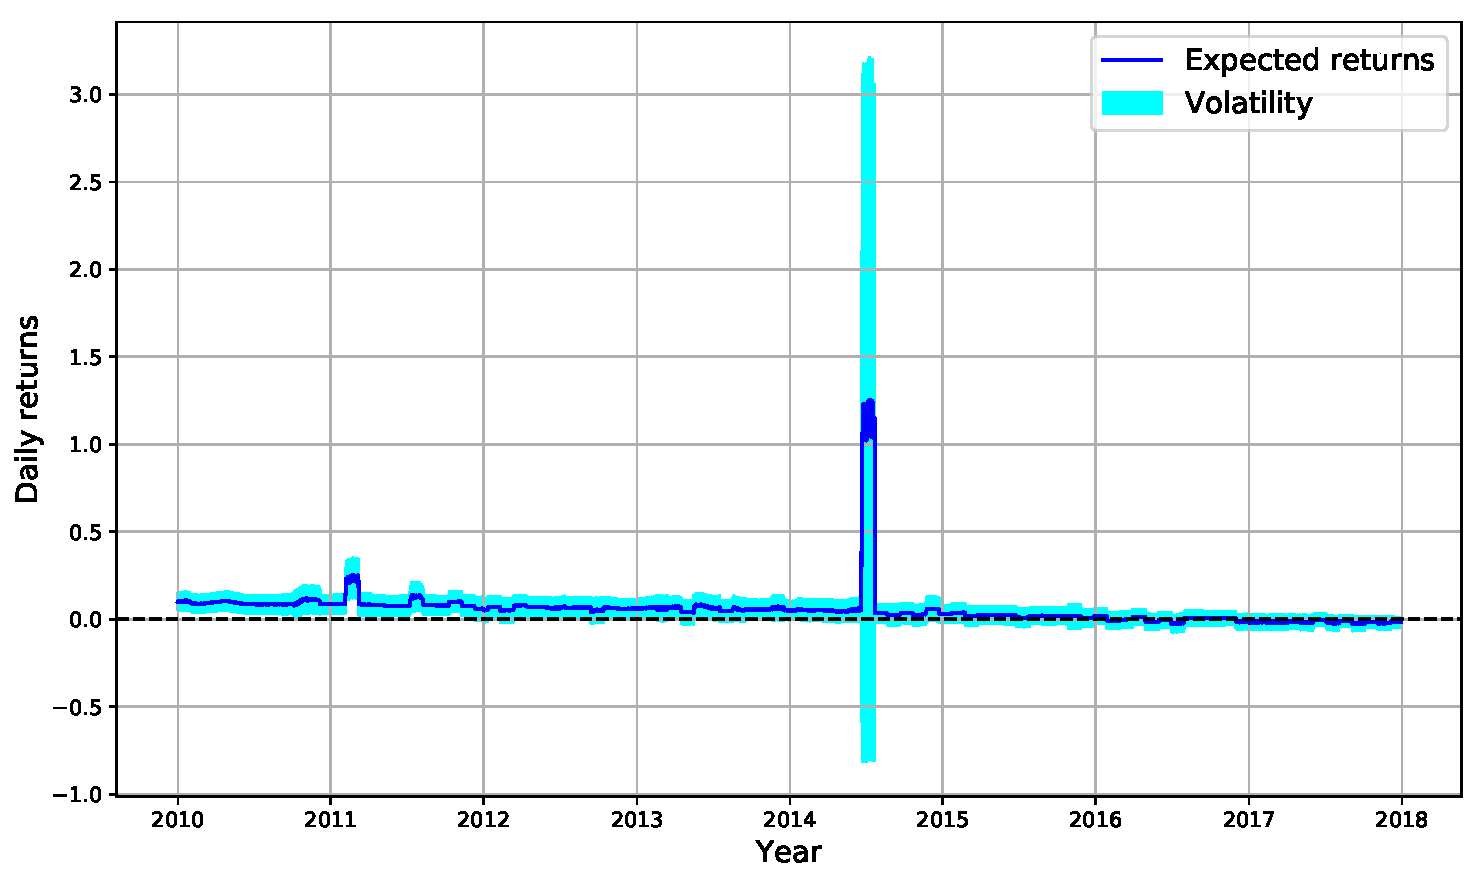
\includegraphics[width=0.75\linewidth]{figures/exp_ret_yearly.pdf}
\caption{Predicted returns for Case I}
\label{fig:ret_yrly}
\end{figure}  

In figure \ref{fig:ret_yrly}, we can observe that the predicted returns are strictly positive from 2010 to 2016. This can be due to the continuous increment of prices in the market. Although, the trend of the returns is decreasing except for peaks in 2011 and 2014. 


\subsection{Case II}
In this case, the performance is computed using a shift of 22 days and the back-test window length of 10 years. The in-sample window of 10 years (starting from 2000-2009) with the step of 22 days is used for calibration and the returns are predicted from 2010 to 2017 sequentially. The predicted returns calculated for period 2010-01-01 to 2017-12-31 are shown in figure \ref{fig:ret_mnthly10}.

\begin{figure}[h!] 
\centering
 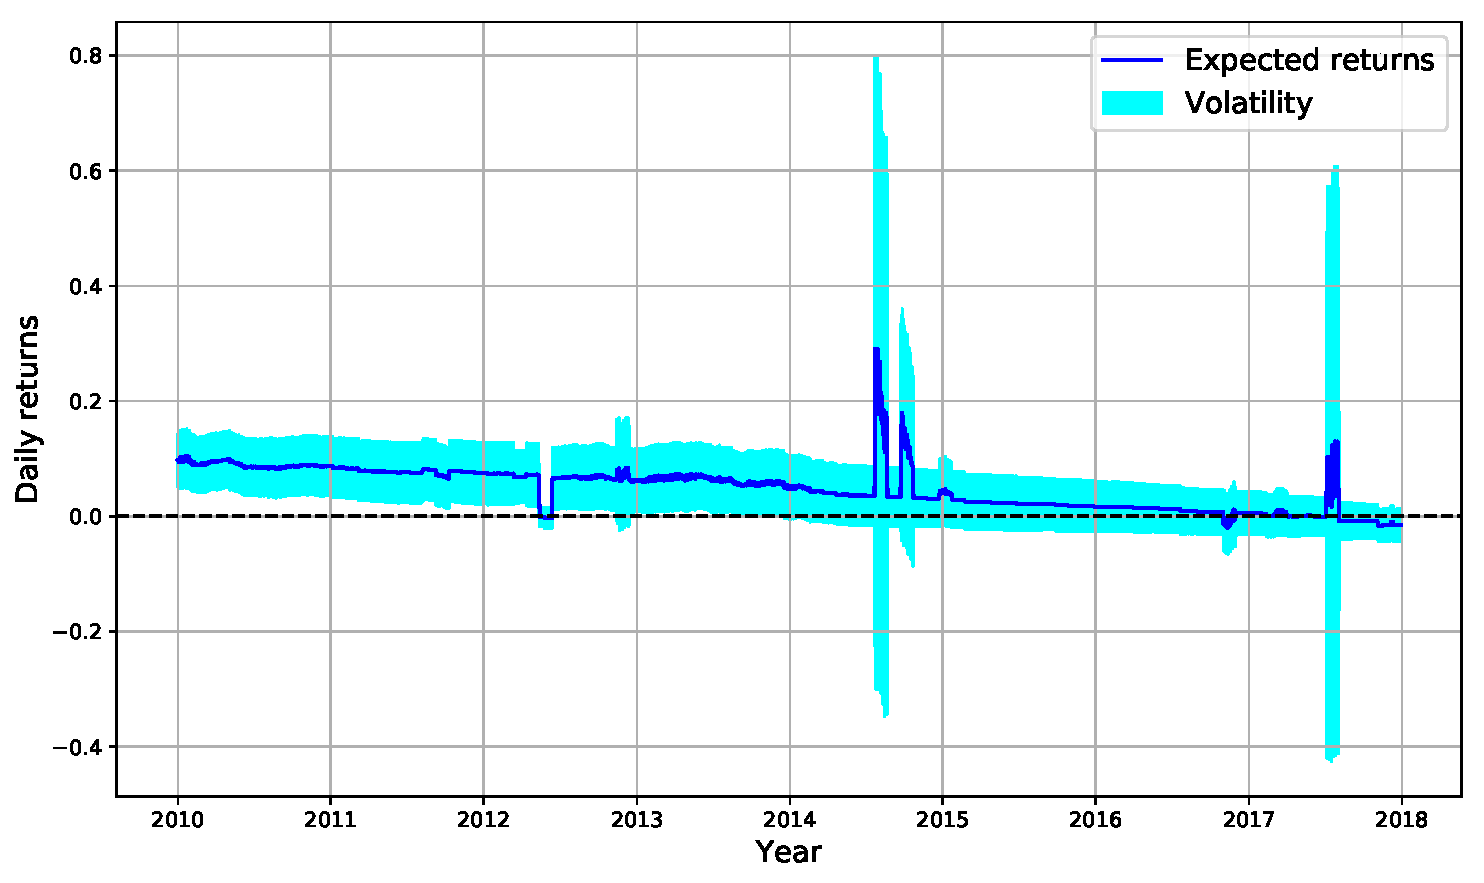
\includegraphics[width=0.75\linewidth]{figures/exp_ret_llf10.pdf}
\caption{Predicted returns for Case II}
\label{fig:ret_mnthly10}
\end{figure}  


In figure \ref{fig:ret_mnthly10}, we can observe that the predicted returns are mostly positive from 2010 to 2016 and follow a decreasing trend. The same behavior is observed for returns for in figure \ref{fig:ret_yrly}. Apart from the similarities, a drawdown in returns can be seen for 2012.


\subsection{Case III}
In this case, the performance is computed using a shift of 22 days and the back-test window length of 10 years. The in-sample window of 5 years (starting from 2000-2004) with the step of 22 days is used for calibration and the returns are predicted from 2005 to 2017 sequentially. The predicted returns calculated for period 2005-01-01 to 2017-12-31 are shown in figure \ref{fig:ret_mnthly5}.

\begin{figure}[h!] 
\centering
 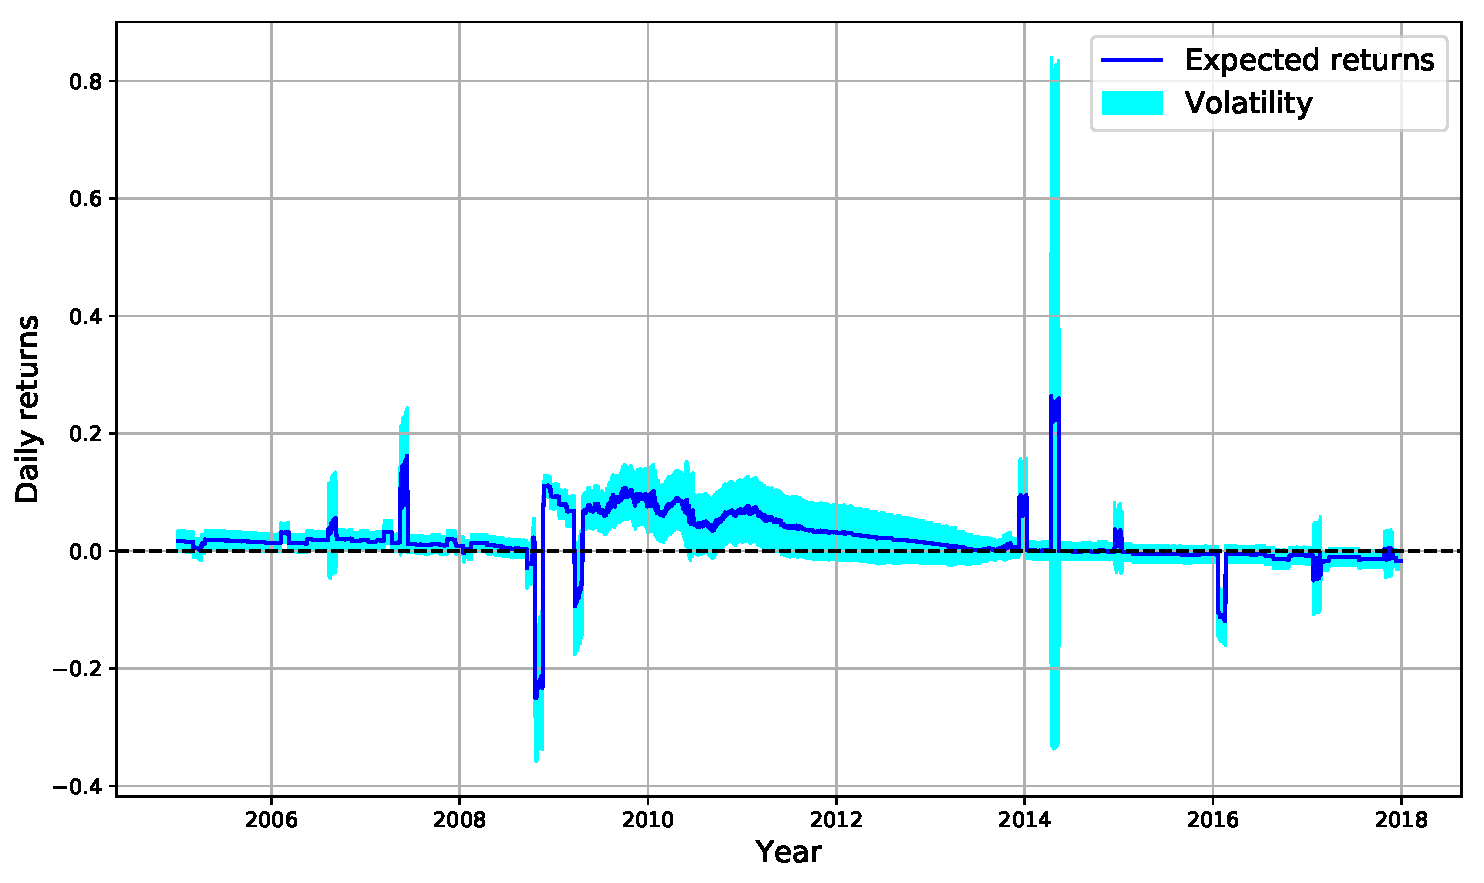
\includegraphics[width=0.75\linewidth]{figures/exp_ret_llf5.pdf}
\caption{Predicted returns for Case III}
\label{fig:ret_mnthly5}
\end{figure}  


In figure \ref{fig:ret_mnthly5}, we can observe that the predicted returns are mostly positive from 2005-2015. We also observe negative returns for period 2008-2009 which seems to be relevant due to the occurrence of the financial crisis in 2008-2009.


\section{Statistical analysis results}
As explained in section 4.1, the next step is to generate a trading signal from predicted returns and volatilities using various trading strategies. We generated signal using two different trading strategies. The first strategy to generate the trading signal ($s(t)$) is given below:
\begin{equation} \label{eqn:signal1}
s(t) = 
\begin{cases}
  Buy\ (+1), & \text{if} \quad r(t) > 0.01 \\
  Short\ (-1), & \text{if} \quad r(t) < -0.01 \\
  Idle\ (0),  & \text{else}
\end{cases}
\end{equation}

The other strategy used is as follow:
\begin{equation} \label{eqn:signal2}
s(t) = 
\begin{cases}
  Buy\ (+1), & \text{if} \quad r(t) > 1*\sigma(t) \\
  Short\ (-1), & \text{if} \quad r(t) < -1*\sigma(t) \\
  Idle\ (0),  & \text{else}
\end{cases}
\end{equation}


We use these strategies to generate a trading signal for predicted returns obtained for all 3 cases. The trading signals and corresponding trading returns calculated using equation \ref{eqn:ret} for first strategy (equation \ref{eqn:signal1}) are shown in figure \ref{fig:t1}, \ref{fig:t2} and \ref{fig:t3}.
Similarly, we generate the trading signal and returns for the strategy explained in equation \ref{eqn:signal2}.

\begin{figure}[h!] 
\begin{tabular}{cc}
\centering 
 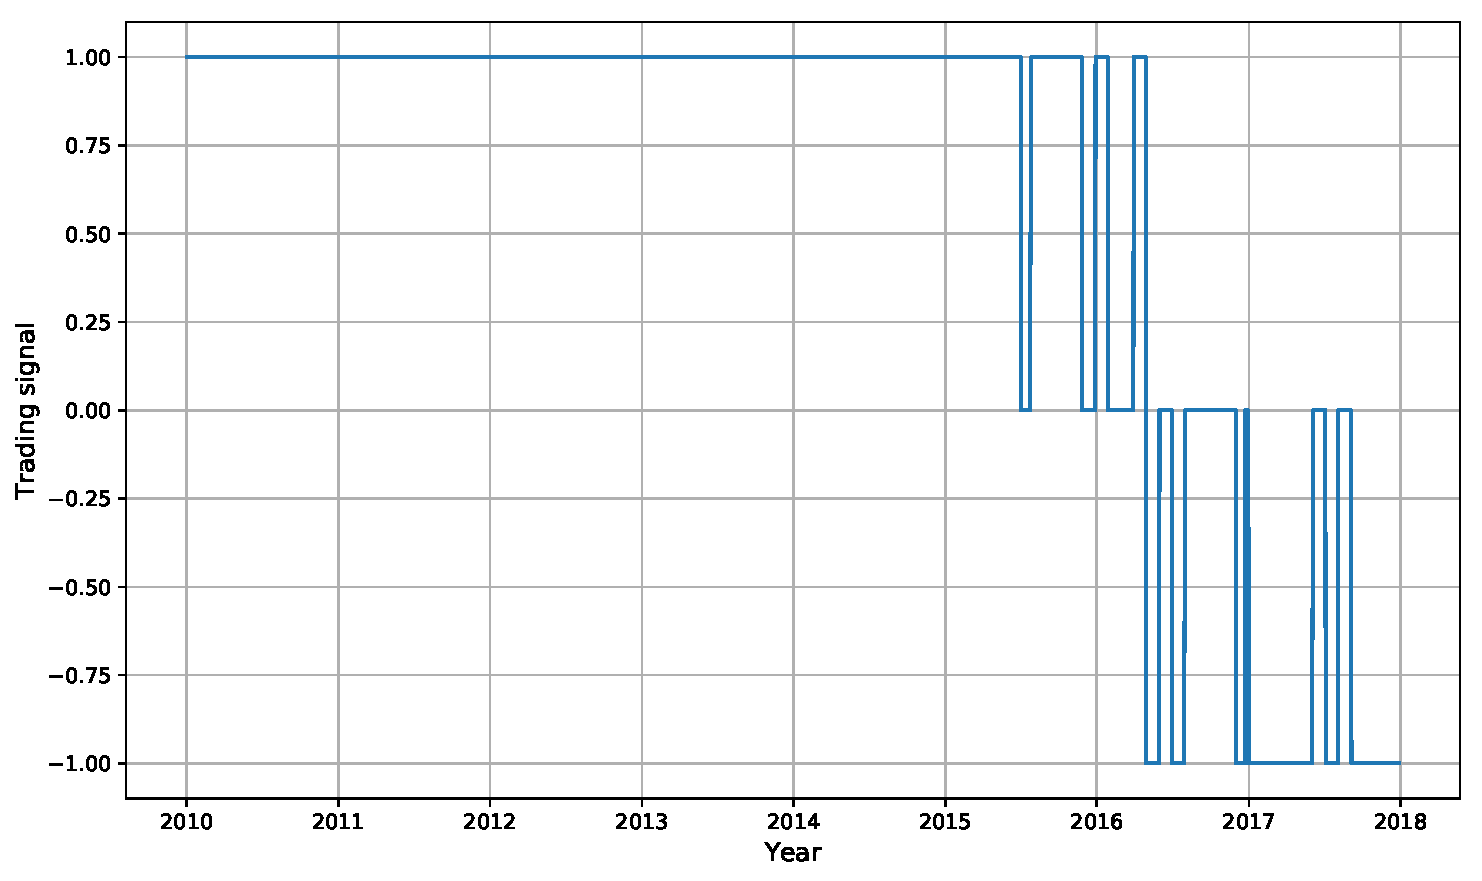
\includegraphics[width=0.5\linewidth]{figures/tradingSig_yearly_llf10.pdf} & 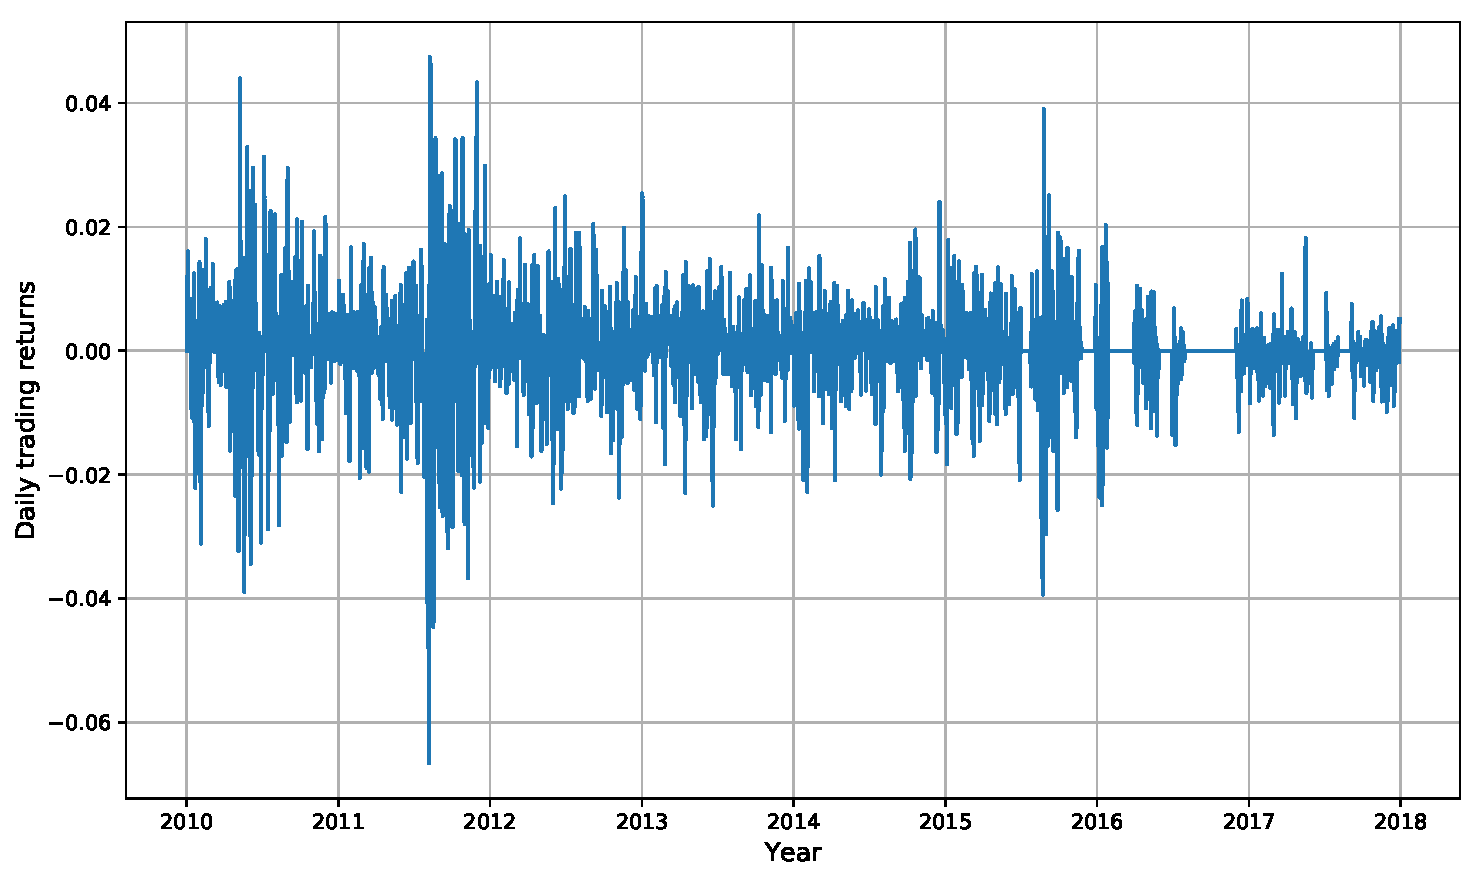
\includegraphics[width=0.5\linewidth]{figures/tradingRet_yearly_llf10.pdf} \\
  (a) & (b)
\end{tabular}
\caption{Results for Case I : (a) trading signal, (b) trading returns}
\label{fig:t1}
\end{figure}



\begin{figure}[h!] 
\begin{tabular}{cc}
\centering 
 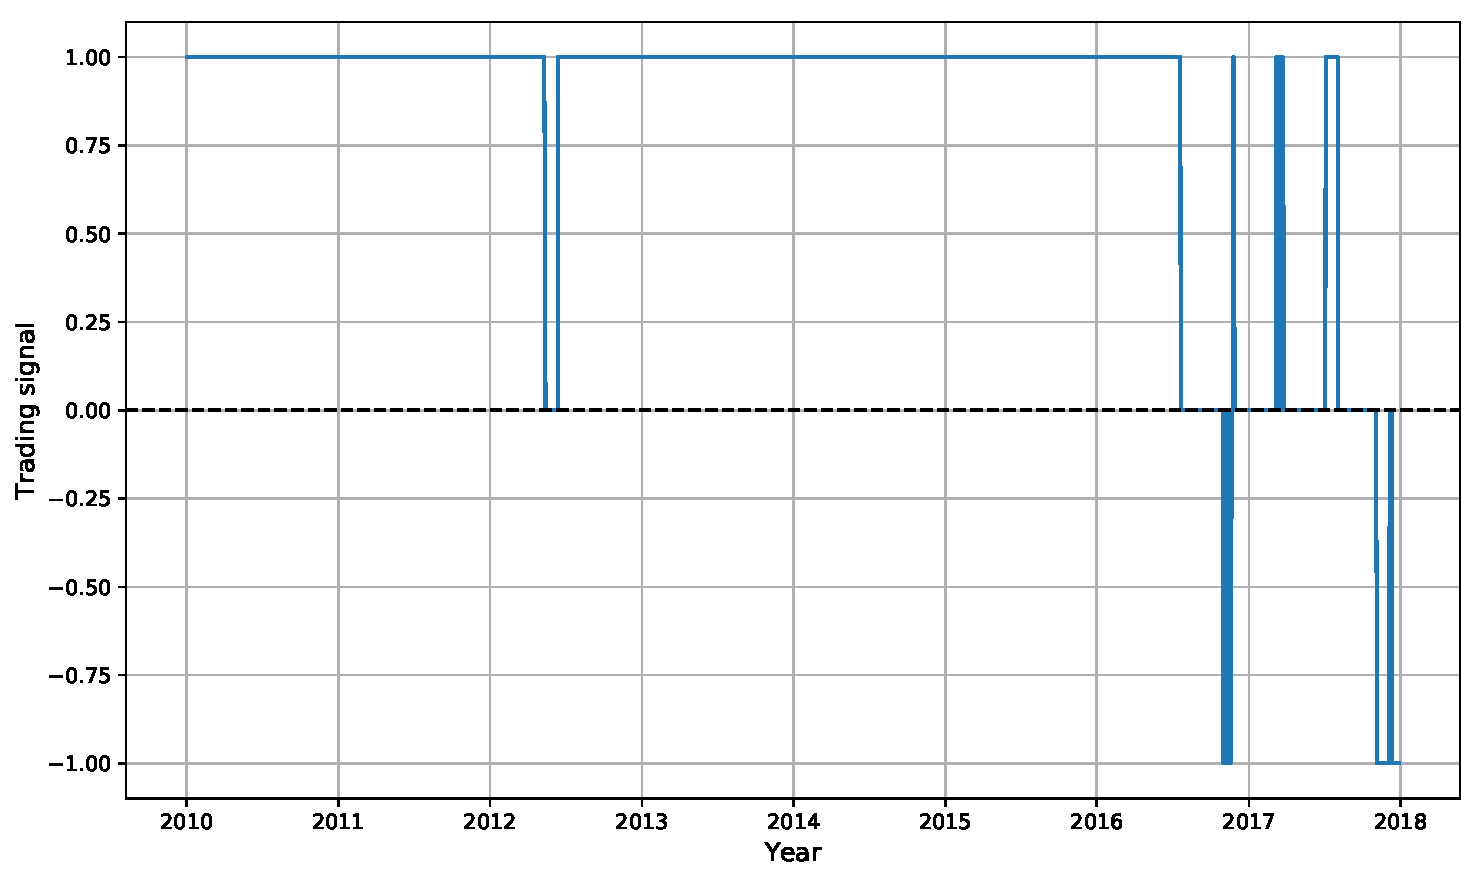
\includegraphics[width=0.5\linewidth]{figures/tradingSig_llf10.pdf} & 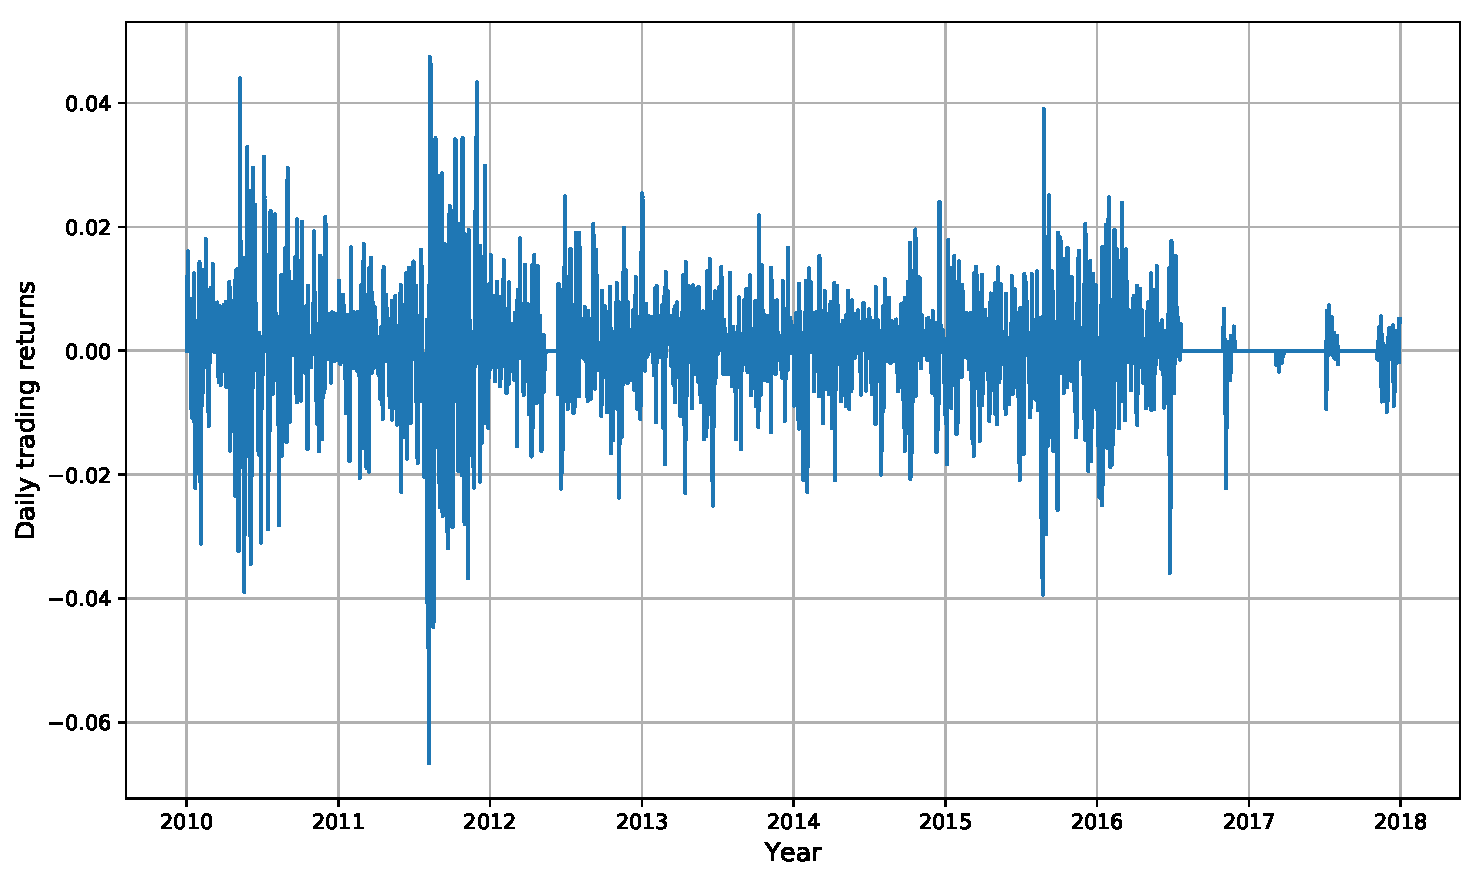
\includegraphics[width=0.5\linewidth]{figures/tradingRet_llf10.pdf} \\
  (a) & (b)
\end{tabular}
\caption{Results for Case II : (a) trading signal, (b) trading returns}
\label{fig:t2}
\end{figure}

\begin{figure}[h!] 
\begin{tabular}{cc}
\centering 
 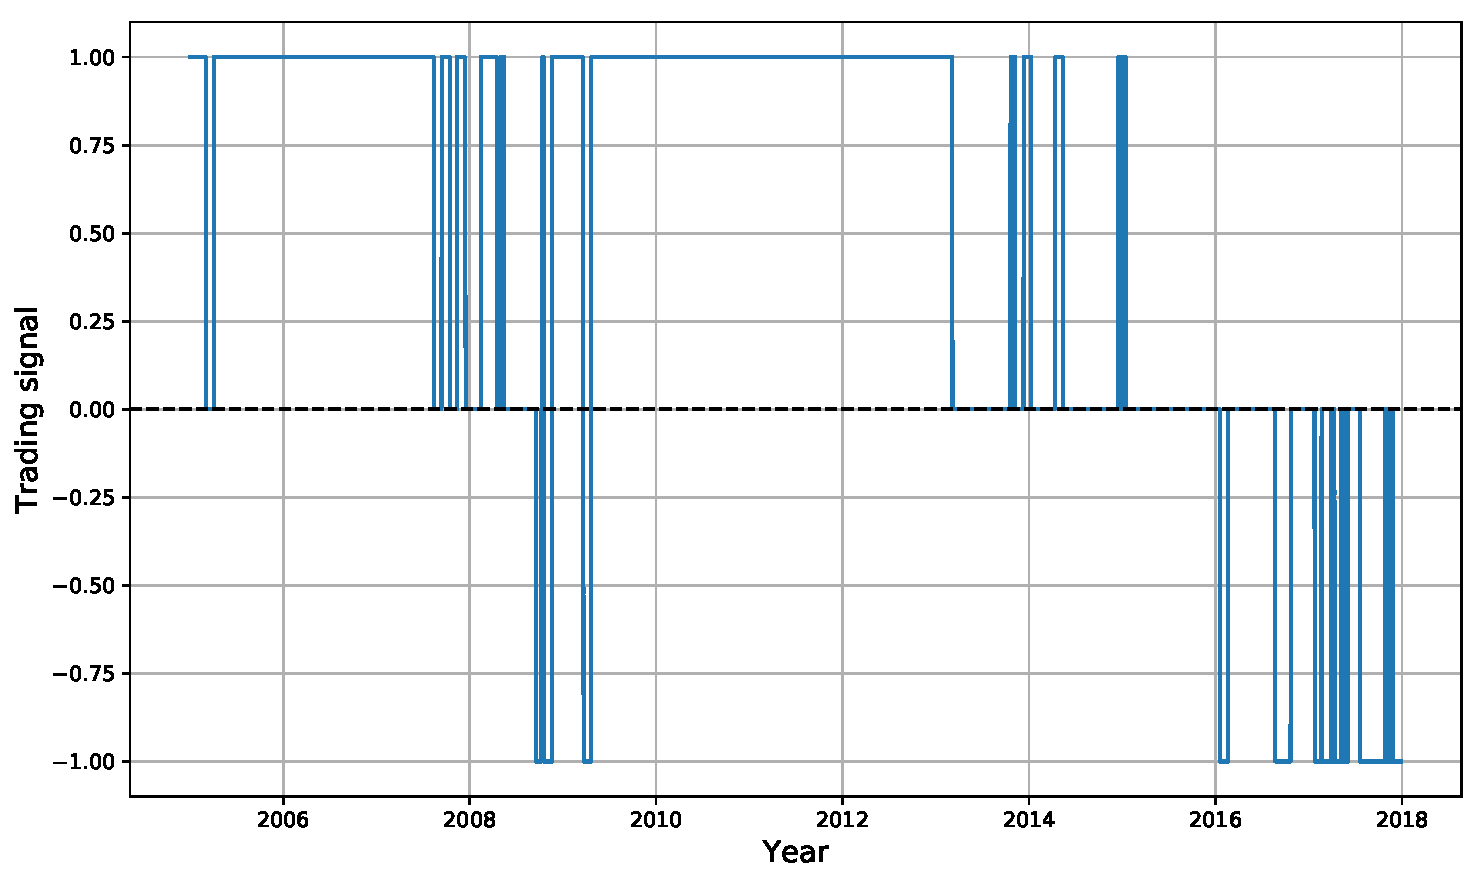
\includegraphics[width=0.5\linewidth]{figures/tradingSig_llf5.pdf} & 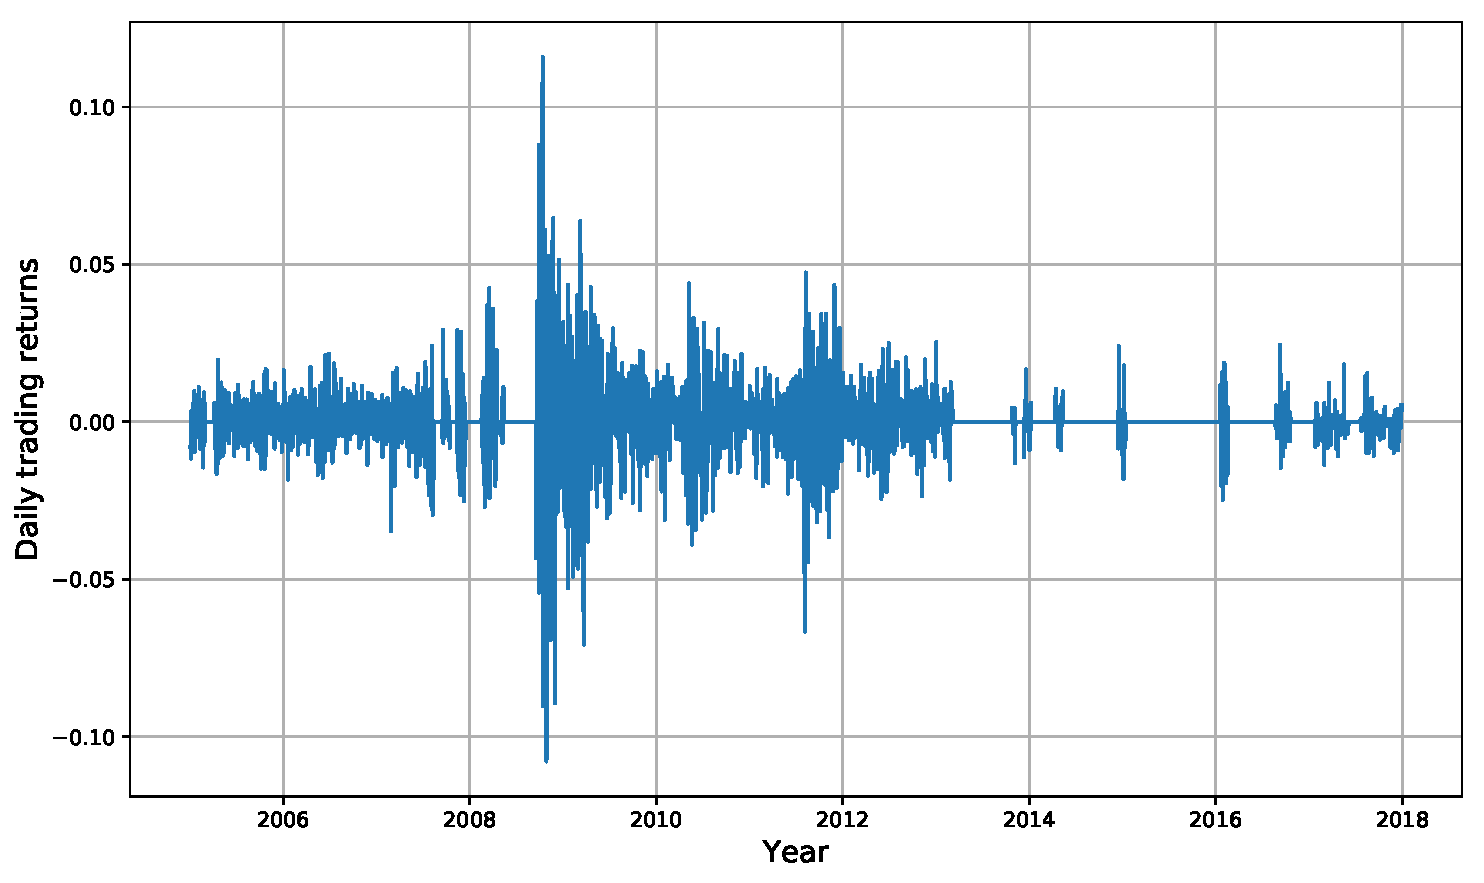
\includegraphics[width=0.5\linewidth]{figures/tradingRet_llf5.pdf} \\
\end{tabular}
\caption{Results for Case III : (a) trading signal, (b) trading returns}
\label{fig:t3}
\end{figure}

\subsection{Comparison with Random strategies}

The model can now be evaluated by comparing SABM trading returns obtained from first trading strategy against returns from randomly generated strategies, as explained in section \ref{ssec:random}. We generated 10,000 random strategies with the constraint of the same number of buy and short days for all the 3 cases. 
The performance of SABM for first strategy in terms of daily Profit and Loss (P\&L) for all the three cases are shown in figure \ref{fig:pnl1}, \ref{fig:pnl2} and \ref{fig:pnl3}. Since the P\&Ls results for the second strategy were not comparable to results from the first strategy, so, further analysis is done using the first strategy only.

\begin{figure}[h!]
\centering 
 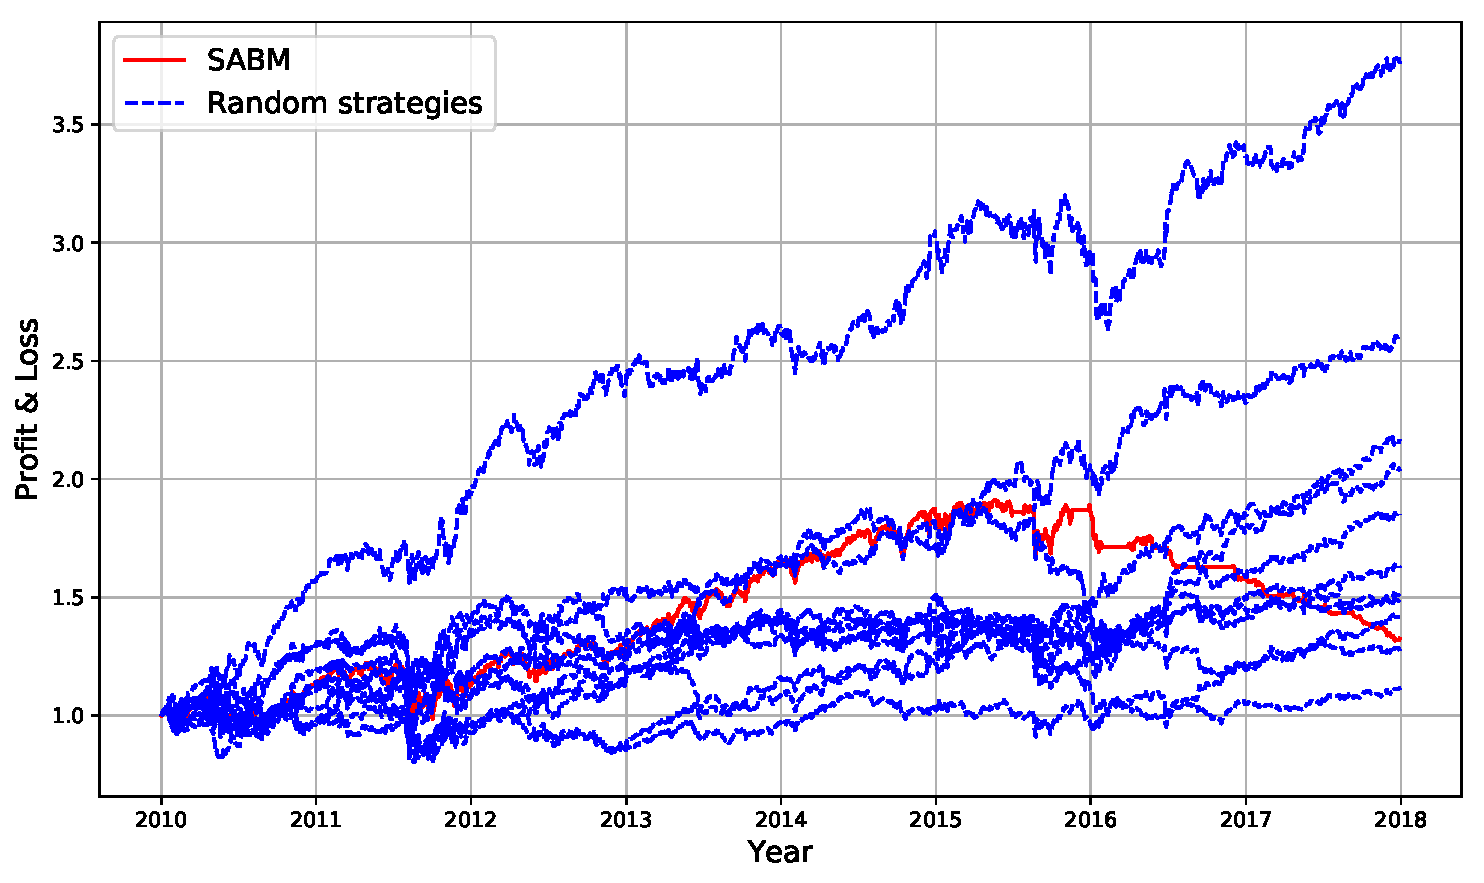
\includegraphics[width=0.75\linewidth]{figures/pnls_yearly.pdf} 
\caption{Daily Profit and Loss for Case I: SABM in red, Random strategies in blue}
\label{fig:pnl1}
\end{figure}

\begin{figure}[h!] 
\centering 
 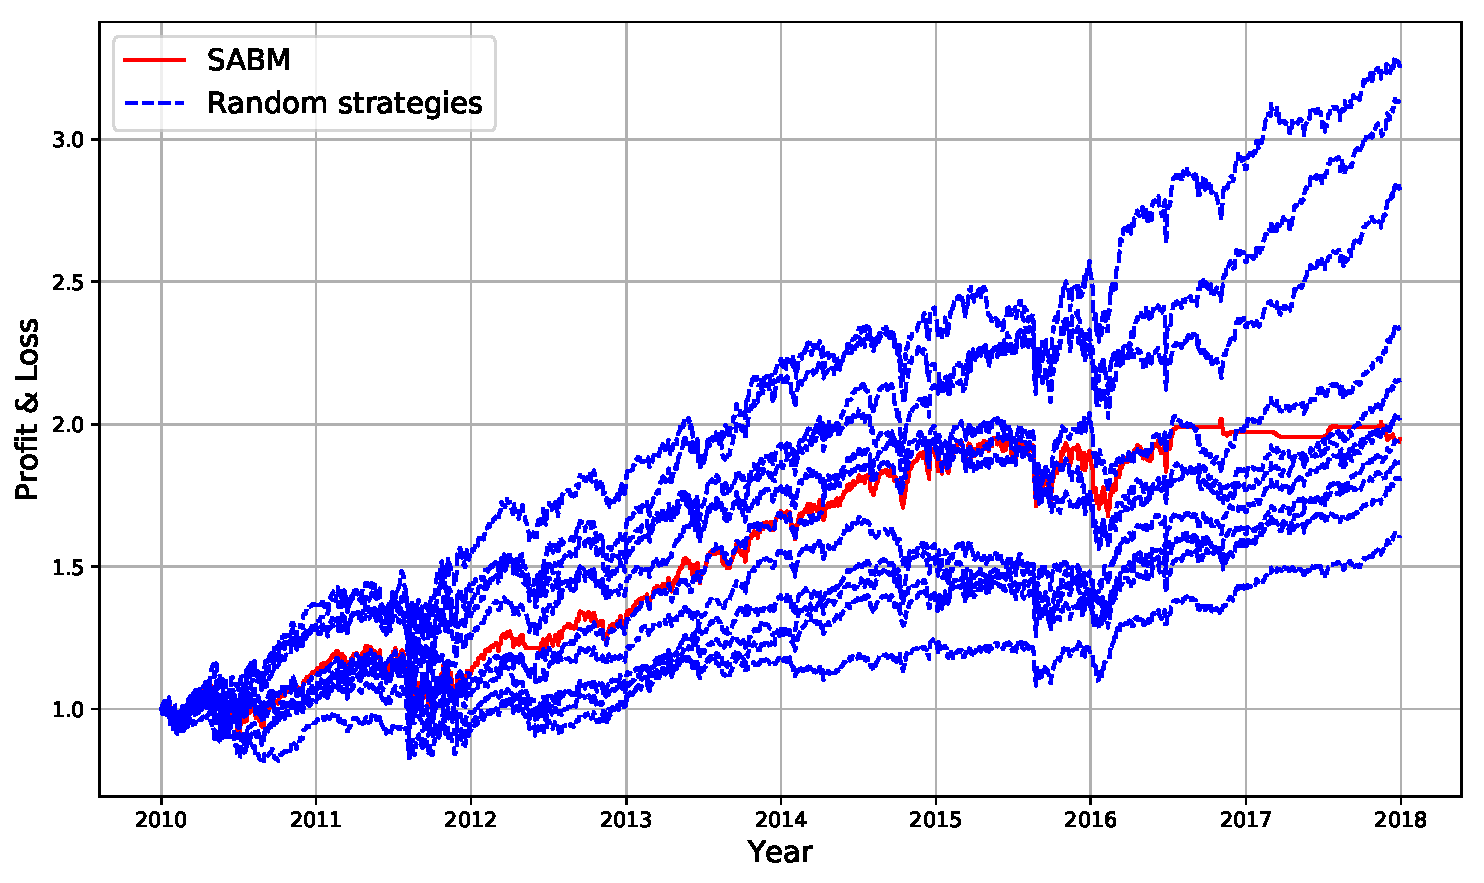
\includegraphics[width=0.75\linewidth]{figures/pnls_llf10.pdf} 
\caption{Daily Profit and Loss for Case II: SABM in red, Random strategies in blue}
\label{fig:pnl2}
\end{figure}

\begin{figure}[h!] 
\centering 
 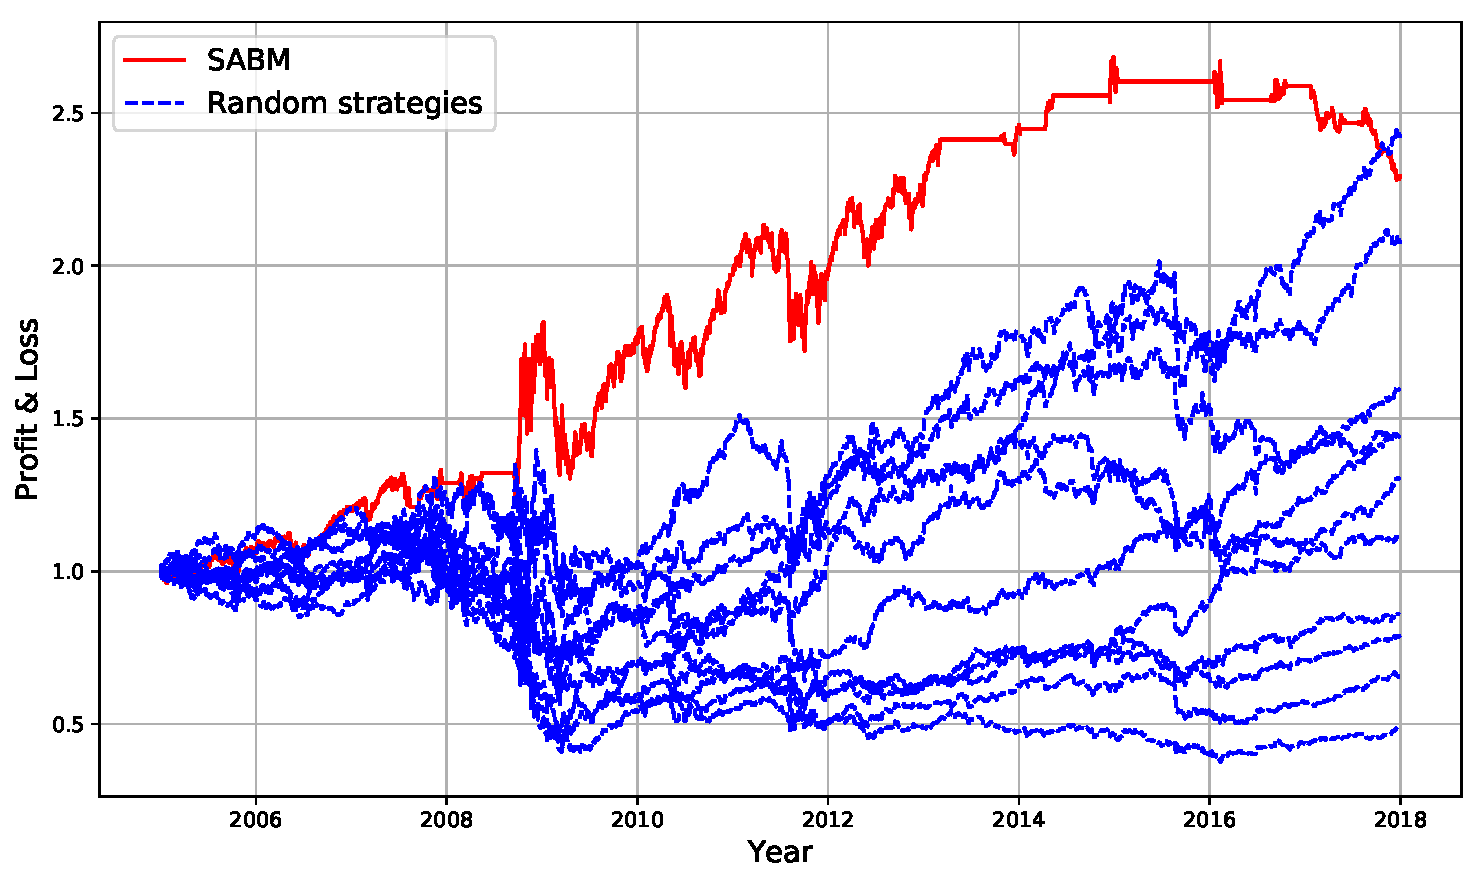
\includegraphics[width=0.75\linewidth]{figures/pnls_llf5.pdf} 
\caption{Daily Profit and Loss for Case III: SABM in red, Random strategies in blue}
\label{fig:pnl3}
\end{figure}

In the P\&L graphs for all 3 cases, the P\&L for Case III is better than the other two cases. In order to validate, we calculate the value of three performance indicators explained in \ref{ssec:random}. These indicators are shown in the table \ref{table:random}. 

\begin{table}[h!]
\begin{center}
\begin{tabular}{|c|cc|cc|cc|}
\hline
    \multicolumn{1}{|c|}{}&  \multicolumn{2}{|c|}{Sharpe ratio} & \multicolumn{2}{|c|}{Maximum drawdown} & \multicolumn{2}{|c|}{CAGR}\\
% \hline
    &  SABM &  Better than(\%) & SABM & Better than(\%) & SABM & Better than(\%) \\
\hline
    Case I &  0.451 &   21.42 &   0.31  &    21.33  & 0.041  & 21.77 \\
    Case II &  0.24 &   37.73 &   0.64  &    64.21  & 0.1    & 44.47  \\
    Case III &  0.393 &   83.3 &   0.457 &    91.8  & 0.072  & 86.31 \\
\hline
\end{tabular}
\end{center}
\caption{Results for different performance indicators}
\label{table:random}
\end{table}

The table \ref{table:random} shows the performance of our model in terms of Sharpe ratio, maximum drawdown, and CAGR for all 3 cases. The performance of our strategy is compared with the performance of random strategies. In case of Sharpe ratio and CAGR, we count the number of random strategies for which the value is less than the value of SABM. This number is shown as a percentage of total strategies in column ``Better than (\%)''. Similarly, for maximum drawdown, the number of random strategies for which the drawdown is more than the drawdown of our SABM, is calculated. We can observe the improvement in percentage for all three indicators for Case III. 


\section{Linear regression}
The other method to evaluate our model is to run linear regression using \textit{FAMA-FRENCH 3 factors model}, as explained in section \ref{ssec:linear}.
We use the trading returns as a dependent variable. The regression was run for all 3 cases. The regression was run using \textit{ols} functionality from \textit{statsmodels} python package. The results for Case I, II and III are shown in figure \ref{table:lr_case1}, \ref{table:lr_case2} and \ref{table:lr_case3} respectively.


\begin{table}
\center
\begin{tabular}{|lc|lc|}
\hline
\textbf{Dep. Variable:}    &     exp\_ret      & \textbf{  R-squared:         } &     0.114   \\
\textbf{Model:}            &       OLS        & \textbf{  Adj. R-squared:    } &     0.113   \\
\textbf{Method:}           &  Least Squares   & \textbf{  F-statistic:       } &     128.7   \\
\textbf{Log-Likelihood:    } &    6775.5 & \textbf{  Prob (F-statistic):} &  2.47e-53   \\
\textbf{No. Observations:} &        2013      & \textbf{  AIC:               } & -1.355e+04  \\
\textbf{Df Residuals:}     &        2010      & \textbf{  BIC:               } & -1.353e+04  \\
\textbf{Df Model:}         &           2      & \textbf{                     } &             \\
\hline
\end{tabular}

\bigskip

\begin{tabular}{|l|cccccc|}
\hline

                   & \textbf{coef} & \textbf{std err} & \textbf{t} & \textbf{P$>$$|$t$|$} & \textbf{[0.025} & \textbf{0.975]}  \\
\hline
\textbf{Intercept} &       0.0002  &        0.000     &     0.947  &         0.344        &       -0.000    &        0.001     \\
\textbf{SMB}       &       0.0046  &        0.000     &    12.882  &         0.000        &        0.004    &        0.005     \\
\textbf{HML}       &       0.0039  &        0.000     &    10.062  &         0.000        &        0.003    &        0.005     \\
\hline
\end{tabular}

\bigskip

\begin{tabular}{|lc|lc|}
\hline

\textbf{Omnibus:}       & 224.686 & \textbf{  Durbin-Watson:     } &    2.035  \\
\textbf{Prob(Omnibus):} &   0.000 & \textbf{  Jarque-Bera (JB):  } & 1629.264  \\
\textbf{Skew:}          &  -0.242 & \textbf{  Prob(JB):          } &     0.00  \\
\textbf{Kurtosis:}      &   7.381 & \textbf{  Cond. No.          } &     2.09  \\
\hline
\end{tabular}
\caption{Regression Results for Case I}
\label{table:lr_case1}
\end{table}



The table \ref{table:lr_case1} shows the value of alpha (excess return) to be 0.02\%, which is positive and insignificant. Also, the coefficients of the two factors, SMB and HML, are positive and statistically significant at 1\% level. The value of $R^2$ is 11.4\%.

\begin{table}
\centering
\begin{tabular}{|lc|lc|}
\hline
\textbf{Dep. Variable:}    &     exp\_ret      & \textbf{  R-squared:         } &     0.137   \\
\textbf{Model:}            &       OLS        & \textbf{  Adj. R-squared:    } &     0.136   \\
\textbf{Method:}           &  Least Squares   & \textbf{  F-statistic:       } &     159.1   \\
\textbf{Log-Likelihood:} &    6768.9 & \textbf{  Prob (F-statistic):} &  7.34e-65   \\
\textbf{No. Observations:} &        2013      & \textbf{  AIC:               } & -1.353e+04  \\
\textbf{Df Residuals:}     &        2010      & \textbf{  BIC:               } & -1.351e+04  \\
\textbf{Df Model:}         &           2      & \textbf{                     } &             \\
\hline
\end{tabular}

\bigskip

\begin{tabular}{|l|cccccc|}
\hline

                   & \textbf{coef} & \textbf{std err} & \textbf{t} & \textbf{P$>$$|$t$|$} & \textbf{[0.025} & \textbf{0.975]}  \\
\hline
\textbf{Intercept} &       0.0004  &        0.000     &     1.975  &         0.048        &     2.55e-06    &        0.001     \\
\textbf{SMB}       &       0.0051  &        0.000     &    14.116  &         0.000        &        0.004    &        0.006     \\
\textbf{HML}       &       0.0045  &        0.000     &    11.446  &         0.000        &        0.004    &        0.005     \\
\hline
\end{tabular}

\bigskip

\begin{tabular}{|lc|lc|}
\hline
\textbf{Omnibus:}       & 226.654 & \textbf{  Durbin-Watson:     } &    2.020  \\
\textbf{Prob(Omnibus):} &   0.000 & \textbf{  Jarque-Bera (JB):  } & 1579.960  \\
\textbf{Skew:}          &  -0.271 & \textbf{  Prob(JB):          } &     0.00  \\
\textbf{Kurtosis:}      &   7.306 & \textbf{  Cond. No.          } &     2.09  \\
\hline
\end{tabular}
\caption{Regression Results for Case II}
\label{table:lr_case2}
\end{table}

 
The table \ref{table:lr_case2} shows the value of alpha to be 0.04\%, which is positive and significant at 5\%. Also, the coefficients of the two factors, SMB and HML, are positive and statistically significant at 1\% level. The value of $R^2$ is 13.7\%.


\begin{table}
\centering
\begin{tabular}{|lc|lc|}
\hline
\textbf{Dep. Variable:}    &     exp\_ret      & \textbf{  R-squared:         } &     0.074   \\
\textbf{Model:}            &       OLS        & \textbf{  Adj. R-squared:    } &     0.074   \\
\textbf{Method:}           &  Least Squares   & \textbf{  F-statistic:       } &     131.1   \\
\textbf{Log-Likelihood:} &    10373. & \textbf{  Prob (F-statistic):} &  1.64e-55   \\
\textbf{No. Observations:} &        3272      & \textbf{  AIC:               } & -2.074e+04  \\
\textbf{Df Residuals:}     &        3269      & \textbf{  BIC:               } & -2.072e+04  \\
\textbf{Df Model:}         &           2      & \textbf{                     } &             \\
\hline
\end{tabular}

\bigskip

\begin{tabular}{|l|cccccc|}
\hline
                   & \textbf{coef} & \textbf{std err} & \textbf{t} & \textbf{P$>$$|$t$|$} & \textbf{[0.025} & \textbf{0.975]}  \\
\hline
\textbf{Intercept} &       0.0003  &        0.000     &     1.647  &         0.100        &    -5.57e-05    &        0.001     \\
\textbf{SMB}       &       0.0042  &        0.000     &    13.358  &         0.000        &        0.004    &        0.005     \\
\textbf{HML}       &       0.0028  &        0.000     &    10.217  &         0.000        &        0.002    &        0.003     \\
\hline
\end{tabular}

\bigskip

\begin{tabular}{|lc|lc|}
\textbf{Omnibus:}       & 903.068 & \textbf{  Durbin-Watson:     } &     2.167  \\
\textbf{Prob(Omnibus):} &   0.000 & \textbf{  Jarque-Bera (JB):  } & 78120.161  \\
\textbf{Skew:}          &   0.243 & \textbf{  Prob(JB):          } &      0.00  \\
\textbf{Kurtosis:}      &  26.933 & \textbf{  Cond. No.          } &      1.78  \\
\hline
\end{tabular}
\caption{Regression Results for Case III}
\label{table:lr_case3}
\end{table}

The table \ref{table:lr_case3} shows the value of alpha (excess return) to be 0.03\%, which is positive and significant at 10\%. Also, the coefficients of the two factors, SMB and HML, are positive and statistically significant at 1\% level. The value of $R^2$ is 7.4\%, which is significantly low.
%% ----------------------------------------------------------------------------
%% ----------------------------------------------------------------------------

\chapter{Conclusion}
We have constructed a Statistical Agent-based model which can be populated by artificial agents i.e. fundamentalists and chartists. This model is developed to understand the complexity of the financial market. It is a new way of solving the macro-level economic problems. Moreover, it tries to overcome the drawback of  Agent-based models. The ABMs are considered to be complex and have non-linear chaotic behavior. Also, they only take micro-level factors into consideration and is quite difficult to calibrate for high dimensional problems.

This thesis shows that SABM is an efficient way to deal with multiple factors due to its layering structure. The layering structure allows us to add multiple agents in the first layer and thus, does not add any complexity to the calibration. The calibration is done in next layer using the real returns for a given in-sample window. The calibration is formulated as an optimization problem using Maximum Likelihood Estimation, which provides the optimal values of the five market parameters. In this thesis, we also observe the advantage of re-calibrating the model to obtain best future predictions. These market parameters are further used for predicting the returns in each out-of-sample window. We generate a trading signal using the predicted returns. This is done by using two different trading strategies. Further, these signals are used to compute trading returns from real returns. 

In order to validate our model, we compare the performance of our model with random strategies on various indicators. We computed various results using different window lengths in which Case III outperforms the random strategies in terms of P\&L, Sharpe ratio, Maximum drawdown, and CAGR. Also, the results of linear regression for Case III are better than other cases. It shows a positive $\alpha$ and significant coefficients for market factors. For Case II and III, the $\alpha$ is statistically significant at 10\%-level which means that the $r(t)$ cannot be
explained by the 3 factors only. Thus, it can be concluded that there is some information in the model.

From these results, we can conclude that the preliminary results are encouraging the prediction. The results can be further improved by performing more experiments. In these experiments, we can select different window lengths, step sizes, and the trading strategies, and do a detailed statistical analysis on the performance of our model.


%% ----------------------------------------------------------------------------
% If Appendix is needed
% %% ----------------------------------------------------------------------------
% \appendix
% %% ----------------------------------------------------------------------------
% BIWI SA/MA thesis template
%
% Created 09/29/2006 by Andreas Ess
% Extended 13/02/2009 by Jan Lesniak - jlesniak@vision.ee.ethz.ch
%% ----------------------------------------------------------------------------
\chapter{Appendix}

\section{Results from Second strategy}




%% add references here

\begin{thebibliography}{99}

\bibitem{ising}
Didier Sornette, "Physics and financial economics (1776–2014): puzzles, Ising and agent-based models", Reports on Progress in Physics, \textit{\url{http://stacks.iop.org/0034-4885/77/i=6/a=062001}}, 2014

\bibitem{a4}
Didier Sornette, Ryan Woodard, Maxim Fedorovsky, Stefan Reimann, Hilary Woodard, Wei-Xing Zhou, "The Financial Bubble Experiment: advanced diagnostics and forecasts of bubble terminations",  arXiv:0911.0454v4 

\bibitem{a5}
Sornette, Didier, and Peter Cauwels. "Financial bubbles: mechanisms and diagnostics", 2014


\bibitem{abm_ref}
Eric Bonabeau, "Agent-based modeling: Methods and techniques for simulating human systems", 2002, \textit{\url{http://www.pnas.org/content/99/suppl_3/7280.full.pdf}}, Proceedings of the National Academy of Sciences

\bibitem{yukalov}
V.I. Yukalov and D. Sornette, "Manipulating decision making of typical agents", \textit{\url{https://pdfs.semanticscholar.org/e1dc/55008178df7f53ad95f5290b5ceaf43153b3.pdf}}

\bibitem{windrum}
Paul Windrum, Giorgio Fagiolo, and Alessio Moneta, "Empirical Validation of Agent-Based Models: Alternatives and Prospects", Journal of Artificial Societies and Social Simulation, \textit{\url{http://jasss.soc.surrey.ac.uk/10/2/8.html>}}, 2007

\bibitem{qunzhi}
Qunzhi Zhang, ``Disentangling Financial Markets and Social Networks: Models and Empirical Tests", PhD thesis at ETH Zurich, 2013

\bibitem{a1}
\textit{\url{http://realinvestmentadvice.com/the-fat-pitch-miss/}}


\bibitem{a2}
\textit{\url{http://www.schroders.com/hu/sysglobalassets/digital/insights/pdfs/hidden-risk-of-going-passive-july-2014.pdf}}


\bibitem{a3}
\textit{\url{https://ftalphaville.ft.com/2017/05/30/2189496/passive-investing-is-worse-than-the-misuse-of-antibiotics/}}

\bibitem{a7}
\textit{\url{https://towardsdatascience.com/probability-concepts-explained-maximum-likelihood-estimation-c7b4342fdbb1}}


\bibitem{a8}
\textit{\url{http://www.epimodels.org/10_Midas_Docs/infoMaterials/MIDAS_101_Model_Types_flyer_web.pdf}}

\bibitem{a9}
\textit{\url{https://www.cairn-int.info/article-E_RFS_554_0653--the-potential-and-limitations-of.htm}}


\bibitem{a10}
\textit{\url{https://www.investopedia.com/terms/c/cagr.asp}}

\end{thebibliography}

% 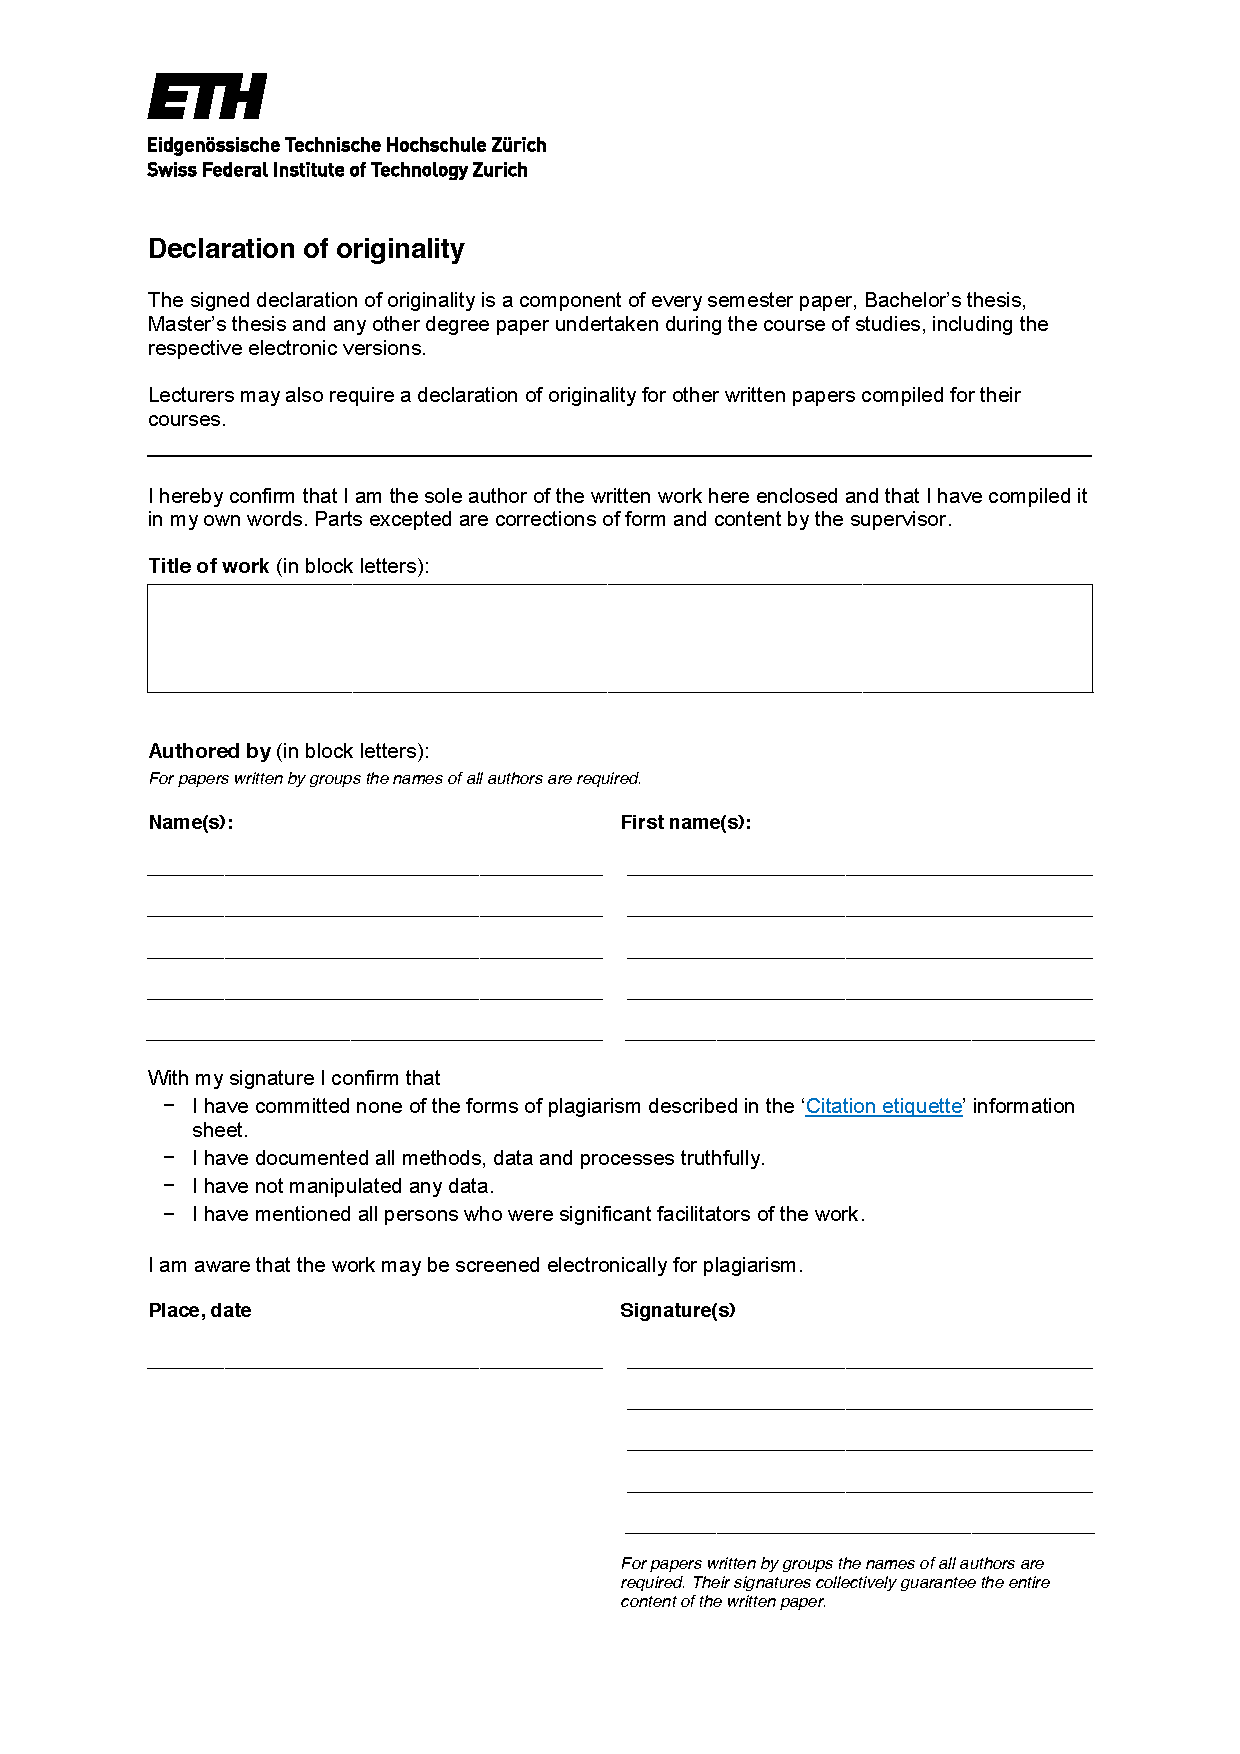
\includepdf[pages={-}]{declaration-originality.pdf}

\end{document}

